\documentclass[phd,icsa,twoside,logo,11pt]{infthesis}

\usepackage{natbib}
\usepackage{graphicx}
\usepackage{listings}
\usepackage{xcolor}
\usepackage{hyperref}
\usepackage{amsmath}
\usepackage{amsthm}
\usepackage{amsfonts}
\usepackage{calligra}
\usepackage[T1]{fontenc}
\usepackage[utf8]{inputenc}
\usepackage{tcolorbox}
\tcbuselibrary{theorems}
\usepackage{mathptmx}

\hyphenpenalty=100000

\newtcbtheorem[number within=section]{definition}{Definition}%
{colback=green!5,colframe=green!35!black,fonttitle=\bfseries}{th}

\definecolor{sh_comment}{rgb}{0.65, 0.00, 0.00 }
\definecolor{sh_keyword}{rgb}{0.15, 0.25, 0.25}
\definecolor{sh_string}{rgb}{0.08, 0.69, 0.08}

\lstset{
float=[*],
language=C,
basicstyle=\linespread{1}\scriptsize\ttfamily,
stringstyle=\color{sh_string},
keywordstyle = \color{sh_keyword}\bfseries,
commentstyle=\color{sh_comment}\itshape,
numbers=left,
numberstyle=\scriptsize,
stepnumber=1,
numbersep=5pt,
backgroundcolor=\color{white},
showspaces=false,
showstringspaces=false,
showtabs=false,
xleftmargin=2em,
frame=lines,
framexleftmargin=1.5em,
framexbottommargin=0em,
prebreak=\space,
postbreak=\mbox{{\color{blue}\scriptsize$\hookrightarrow$}},
breaklines=true,
breakatwhitespace=false,
tabsize=2,
captionpos=b,
escapeinside={([}{])},
language=C++
}

\lstdefinelanguage{CAnDL}
{
morekeywords = {Constraint, with, opcode, collect, include, function\_name, data\_type, ir\_type, domination, strict\_domination, calculated\_from, control\_origin, data\_origin, End },
morecomment  = [s]{\{}{\}}
}

\title{Idiomatic Code Acceleration for Heterogeneous Systems}
\author{Philip Ginsbach}

\abstract{%
    This doctoral thesis will present the results of my work into the
    reanimation of lifeless human tissues.
}

\begin{document}
\begin{preliminary}
\maketitle
\begin{acknowledgements}
First and foremost I want to thank Mike for his ...
\end{acknowledgements}
\begin{declaration}
    I declare that this thesis was composed by myself, that the work contained
    herein is my own except where explicitly stated otherwise in the text, and
    that this work has not been submitted for any other degree or professional
    qualification except as specified.
    Some of the material used in this thesis has been published in the following
    papers:
    \begin{itemize}
        \item Philip Ginsbach and Michael F.\ P.\ O'Boyle.
              ``{\bf Discovery and Exploitation of General Reductions: A Constraint
                Based Approach}''.
              In: {\em Proceedings of the 15th Annual International
                  Symposium on Code Generation and Optimization (CGO), 2017}
        \item Philip Ginsbach, Lewis Crawford and Michael F.\ P.\ O'Boyle.
              ``{\bf CAnDL: A Domain Specific Language for Compiler Analysis}''.
              In: {\em Proceedings of the 27th International Conference on
                  Compiler Construction (CC), 2018}
        \item Philip Ginsbach, Toomas Remmelg, Michel Steuwer, Bruno Bodin,
              Christophe Dubach and Michael F.\ P.\ O'Boyle.
              ``{\bf Automatic Matching of Legacy Code to Heterogeneous APIs: An
              Idiomatic Approach}''.
              In: {\em Proceedings of the 23rd International Conference on
                  Architectural Support for Programming Languages and Operating
                  Systems (ASPLOS), 2018}
        \item Philip Ginsbach, Bruce Collie and Michael F.\ P.\ O'Boyle.
              ``{\bf Automatically Harnessing Sparse Acceleration Libraries}''.
              In: {\em ???, 2019}
    \end{itemize}
    \par
\vspace{1in}\raggedleft({\em Philip Ginsbach})
\end{declaration}
\tableofcontents
\end{preliminary}

\chapter{Introduction}
    The end of Moores Law and the end of Dennard Scaling require new approaches in
    hardware.

    Heterogeneous computing platforms are the natural reaction to this.

    However, with heterogeneous hardware becoming an essential core of computing
    capabilities, thinking of it as library accelerators becomes wrong.

    We need a new hardware software contract instead and heterogeneous hardware
    should become a responsibility of the compiler.

    While compilers have lagged behind the developments in the hardware domain, we
    can profit from experience with multi-core processors.

    Auto-parallelizing compilers have failed to solve the problems and have only had
    major success for specific kernels and using auto-tuning.

    Heterogeneous computing is a superset of parallel computing and so an approach
    to fully automatically optimize code is unlikely.

    At the same time, a library and DSL based approach has been successful, however
    fails to become mainstream due to adoption cost.

    What is promising therefore is a combination of hand-optimized and -parallelized
    libraries together with compiler automatisms.

    This is what we consider an idiomatic approach.

\chapter{Computational Idioms}

    The concept of computational idioms has been observed in different contexts
    and remains a rather vague concept.
    While terms such as \texttt{reduction}, \texttt{stencil} and
    \texttt{linear algebra} are commonly used, the concrete concepts can be
    surprisingly vague, although previous work has established several formal
    approaches.
    We will not try to create our own formal definitions in this chapter, but
    instead want to give an overview of the literature that sheds different
    perspectives on this topic.

    The basic observation is that software programs don't cover the possible
    programs evenly, instead, they tend to be structured among certain design
    principles.
    The same is true algorithmically and particularly for performance intensive
    applications.

\section{Literature Survey}
\subsection{Algorithmic Skeletons}

\subsection{Berkeley Parallel Dwarves}
\subsection{Computational Patterns}

\section{Idiom Specific Optimizations}

\subsection{Important Approaches}
\subsection{Ways of Encapsulating Expertise}


\chapter{Contraint Programming on Static Single Assignment Representation}

\section{Introduction}

    In this chapter we want to lay out a basic methodology to formally describe
    and recognise algorithmic structures in programs during compilation.
    During the different compilation stages, modern optimizing compilers for
    proceedural languages such as C/C++, Fortran or JavaScript typically use
    a range of different representations of the user program.
    Static single assignment (SSA) form has emerged as a suitable representation
    for applying complex optimizing transformations in the mid end.
    It respresentation abstracts away the complexities of both the source
    language and the target architecture, enabling reliable analysis and
    platform independent reasoning.

    Prominent examples of compilers that utilize static single assignement
    representations for the bulk of their optimisation passes are
    {\bf clang/clang++} (LLVM IR), {\bf gcc} (GIMPLE), {\bf v8 Crankshaft}
    (Hydrogen) and {\bf SpiderMonkey} (IonMonkey/MIR).

    The precise instruction set, syntax and type systems of the different static
    single assignment form intermediate representations vary depending on the
    requirements of the source languages (static or dynamic) and the operating
    constraints (JIT or AOF).
    However, they share the same fundamental paradigmes and we can mostly
    abstract away the differences as implementation specific details in this
    chapter.
    Fundamentally, a program in single static assignment form is made up of
    functions that are represented as sequences of instructions that are grouped
    into basic blocks and that operate on virtual registers.
    These virtual registers can be assigned only once and the place of
    assignment can be statically determined.
    In order to support control flow divergence, SSA form utilized PHI nodes
    that enapsulate the non-SSA behaviour.

    In this chapter, we will derive a methodology to recognise structures in 
    SSA code via constraint programming.
    For this to work, we need to develop a mathematical model of it.

\subsection{Static Single Assignment Form}

    Static single assignemnt form is a property that applies to compiler
    intermediate representations.
    Functions in SSA form are represented as sequences of instructions that
    operate on an abstract machine and that are grouped into basic blocks.
    The abstract machine provides an unlimited number of registers and a well
    defined instruction set.
    Each instruction has a finite amount of input arguments and an opcode that
    refers to a specific operation to be performed.
    instruction arguments can be registers or constants and instructions can
    write their result into a single output register.
    Control flow is expressed as branch instructions that can redirect control
    conditionally or unconditionally to the start of other basic blocks.
    Branch instructions signify the end of a basic block.
    Instructions and registers may be statically typed.


    The static single assignemnt property stipulates that within a function,
    each register is only written at a single static location.
    This implies that the data dependencies between the instructions are
    explicit and registers can be identified directly with the instructions that
    write to them.
    The registers themselves can therefore be considered implicit, with only the
    data flow between instructions required to recover them.

    In the presence of dynamic control flow behaviour in the program, most
    simply in the case of a conditional branch, the static single assignment
    property can only be maintained using phi instructions.
    These are particular pseudo-instructions that encapsulate assignments that
    can only dynamically be determined.

\section{Deriving a Mathematical Model}


\begin{figure}[p]
\centering
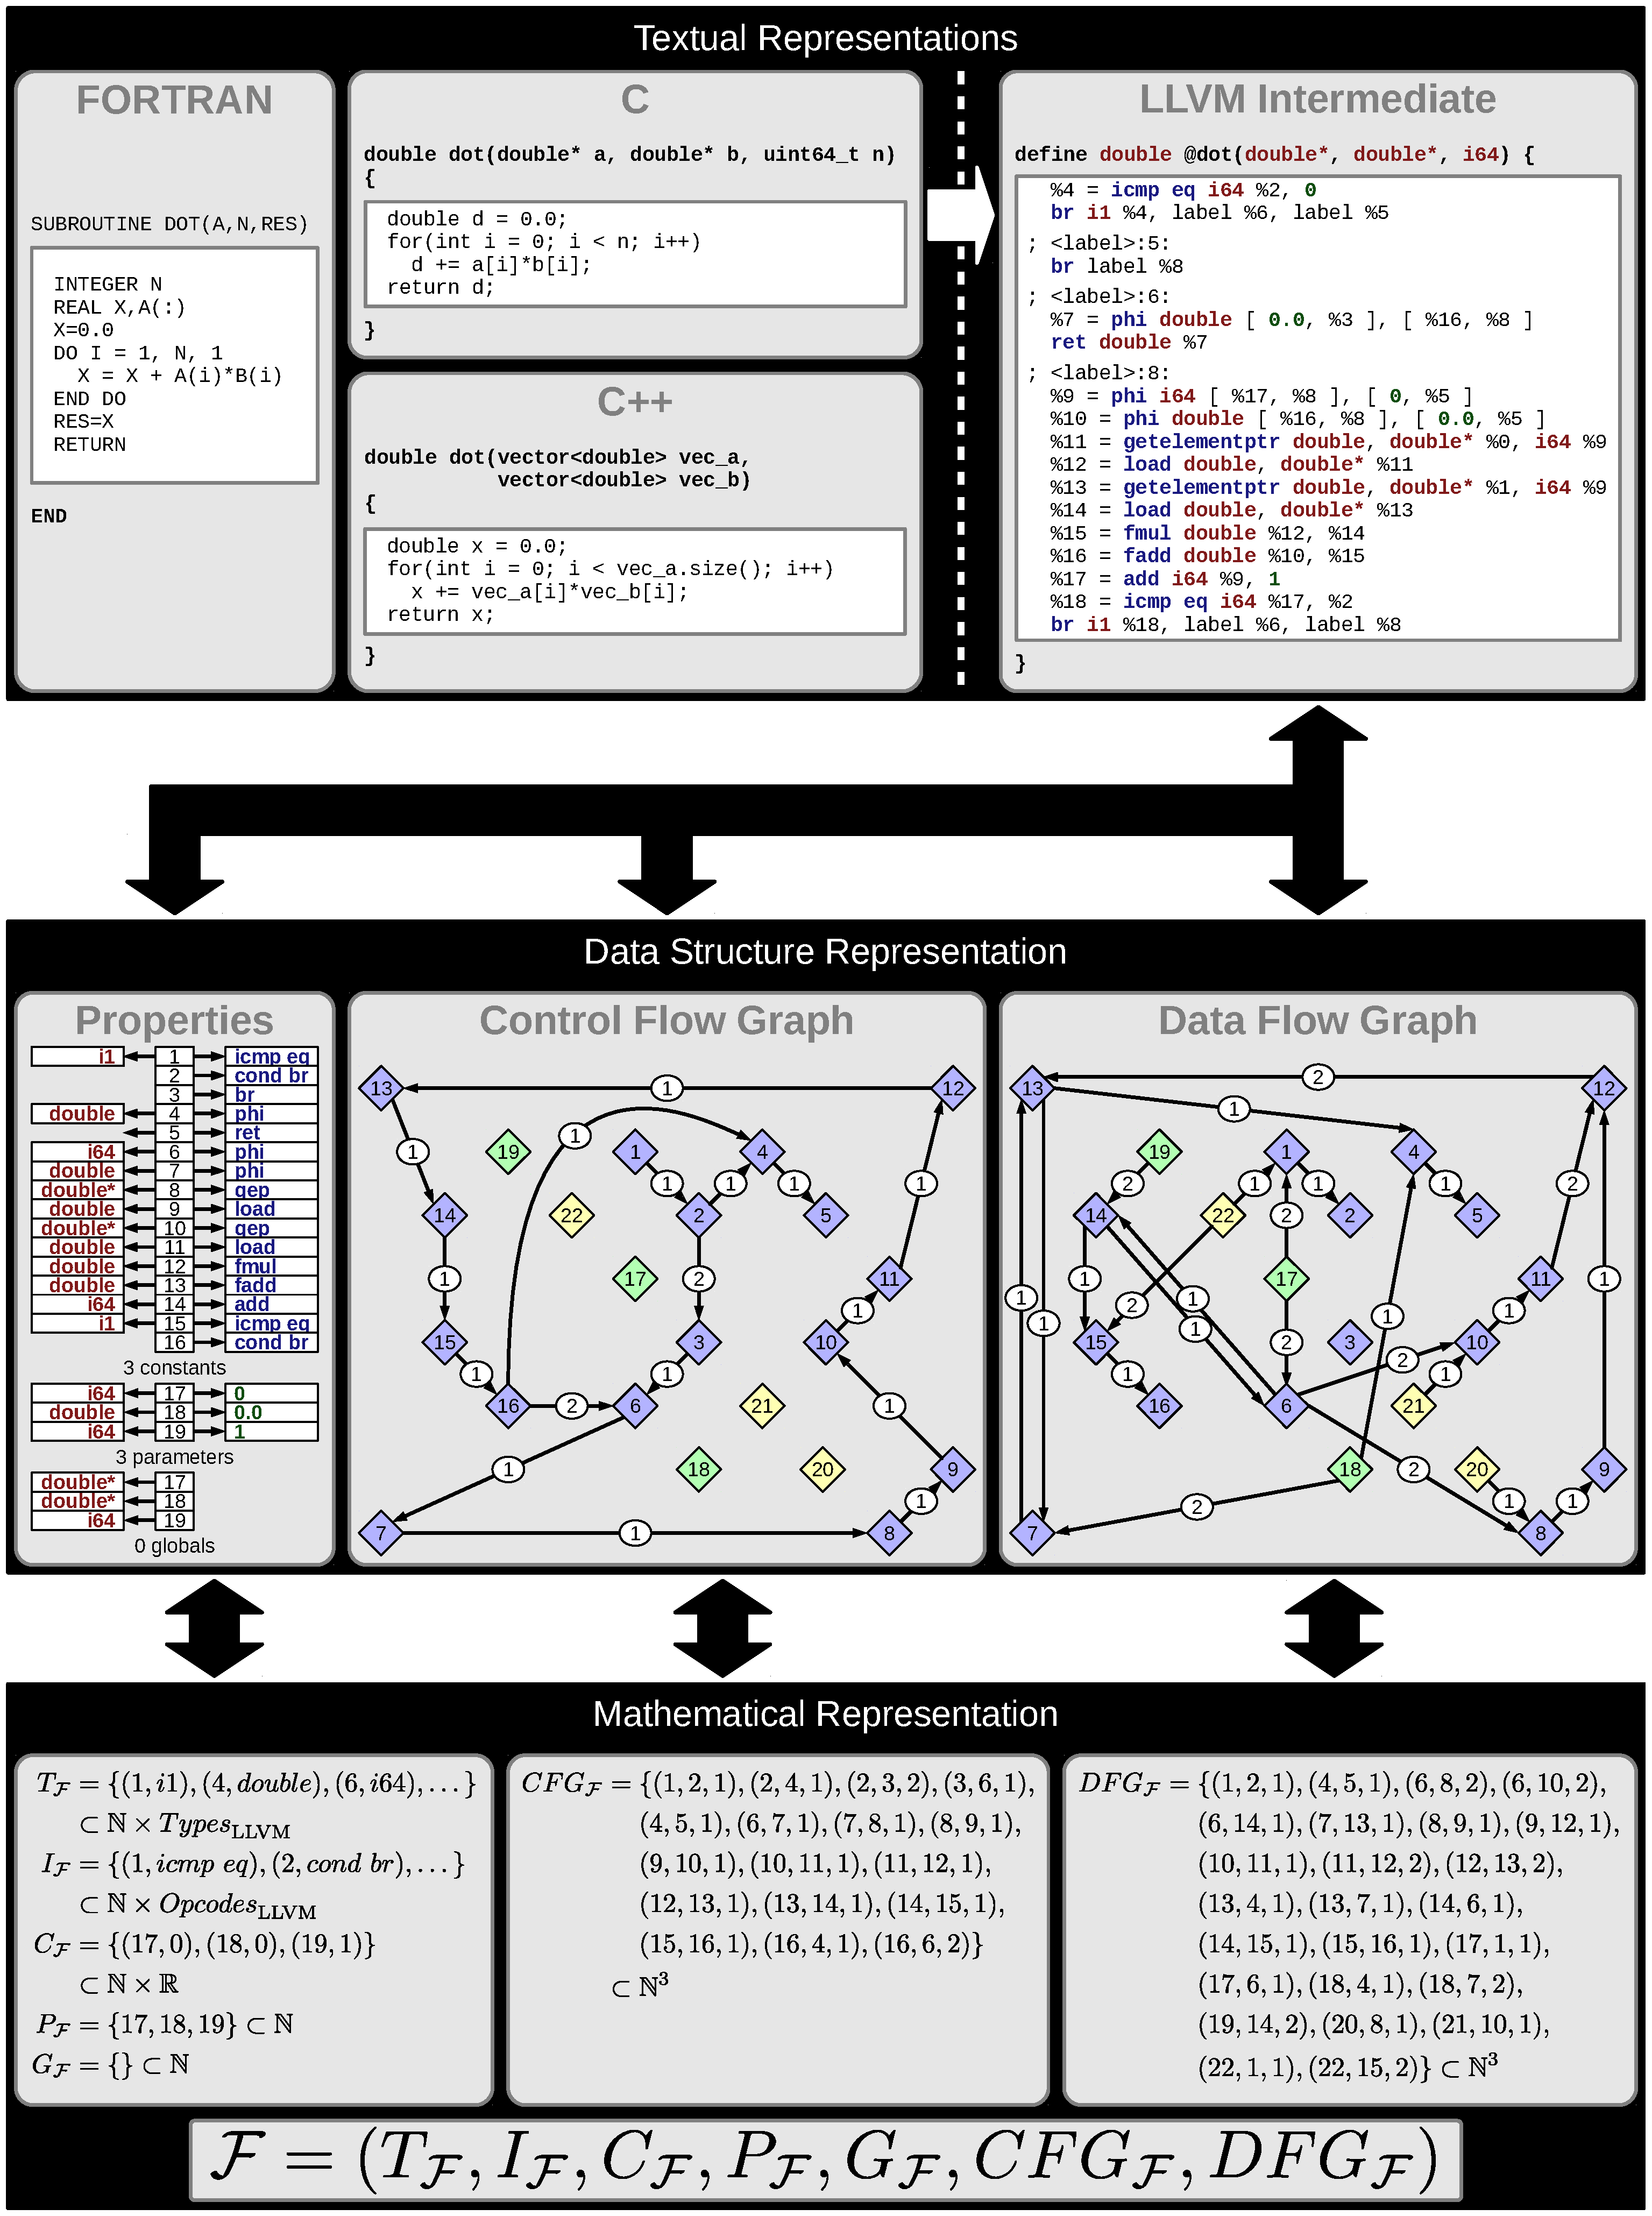
\includegraphics[width=\linewidth]{figures/schaubild.pdf}
\caption{Mathematical descriptions of example source code are derived via graph
         structures of compiler intermediate representation in single static
         assignment form.}
\label{fig:derivemaths}
\end{figure}


    In this section, we will derive a mathematical model of programs in single
    static assignemnt form.
    This will give us a sound basis and mathematical notation for compiler
    analysis problems.
    We will then in later chapters use this to define computational idioms
    formally, and in order to implement automatic compiler tools.
    It is not our aim to introduce a formal operational semantics, or more
    generally to derive a model for the execution of SSA programs.
    Instead, we will describe their static structure, focusing on clear notation
    of the commonalities of existing SSA intermediate representations.

    We discussed in the previous section how SSA representations can be disected
    into different components, including control flow, data flow and instruction
    specifications.
    In \autoref{derivemaths}, we can see how this can be taken further in order
    to extract a more mathematical approach.
    At the top of the figure, we can see different textual representations of a
    simple vector dot product.
    The version of the top right is in an SSA intermediate representation: LLVM
    IR as generated by the clang compiler.

    In the middle column of \autoref{derivemaths}, the information that is
    contained in the SSA representation is split into three components:
    Firstly, the we need a set of per-instruction properties, such as
    instruction opcodes, types and the values of constants that are used.
    Secondly, we capture the control flow graph.
    Thirdly, we capture the detailed data flow graph of the program.
    This data structure contains information about how the results of previous
    instructions are used as arguments to successive instructions.
    As we discussed in the previous section, the SSA property ensures that this
    is enough information to make the concrete register usage implicit.

    We can see this \autoref{derivemaths}.
    The single static assignment property implies that it is statically knows
    at each point, which instruction produced the value in each register.
    Therefore, we can immediately identify registers with their producting
    instruction.
    Therefore we can entirely capture the interaction between instructions in
    two graphs: the control flow graph and the data flow graph.
    This is shown in in middle section of the figure.
    The data flow graph entirely replaces the concept of registers and instead
    models directly how the results from instructions are used as arguments
    in succeeding instructions.
    The control flow graph models the possible paths through the program.

    Note that we entirely removed the concepts of basic blocks and registers
    here.
    However, both can be recovered easily from the graph representations and
    hence we lost no information going from the textual representation towards
    the graph representations.

    Finally, we can model this entirely mathematical.
    We can see at the bottom of the figure, how we can model the entire function
    body as a tuple
    \begin{align*}
        \mathcal{F}=(T_\mathcal{F},I_\mathcal{F},C_\mathcal{F},P_\mathcal{F},G_\mathcal{F},CDG_\mathcal{F},DFG_\mathcal{F})\text{.}
    \end{align*}

    Note that the same model can be used abstractly for other single static
    assignment forms, only the type and opcode information as encoded via
    $Types_\text{LLVM}$ and $Opcodes_\text{LLVM}$ are specific to LLVM and need
    to be replaced.

\newpage

\subsection{Important Graph Properties}

    With our established notation, we can now transfer standard compiler
    analysis problems into this more formal language.
    Most of these properties are based on graph theoretic considerations, so we
    will firstly need to recapitulate some graph theory basics.
    Firstly, there is the notion of {\em cuts} of graphs, that we will introduce
    here in a hybrid version of edge based and vertex based modelling.

    \begin{definition}{Connections and Cuts}{def:cuts}
        Consider an adjacency set $E\subset\mathbb{N}\times\mathbb{N}$ of a
        directed graph and let $a,b\in\mathbb{N}$.
        \newline
        A {\em connection} between $a$ and $b$ in $E$ is a subset
        $A\subset\mathbb{N}$ such that a finite sequence $c_1,\dots,c_n$
        exists with
        \begin{gather*}
            a=c_1\hspace{1cm}c_2,\dots,c_{n-1}\in A\hspace{1cm}b=c_n\\
            (c_k,c_{k+1})\in E\hspace{1em}\text{for all}\hspace{1em}k=1,\dots,n-1.
        \end{gather*}
        A {\em cut} between $a$ and $b$ in $E$ is a subset $B\subset E$
        such that no {\em connection} between $a$ and $b$ in $E\setminus B$
        exists.
        We define the {\em set of cuts} between $a$ and $b$ in $E$ as
        \begin{align*}
            \text{Cuts}_E(a,b):=\{B\subset E\mid B\text{ is {\em cut} between $a$ and $b$ in $E$}\}
        \end{align*}
    \end{definition}

    These notions are quite intuitive, two vertices in a graph have a connection
    if one can reach the other via the available edges and by ``cutting'' these
    edges, they are no longer connected.

    These definitions are very useful in order to identify crucial properties of
    data and control flow graphs.
    Most standard is the the definition of a dominator in the control flow
    graph: An instruction $d$ is said to dominate another instruction $n$ if
    every path from the entry node to $n$ through the control flow graph must
    go through $d$.
    In our model this is of course equivalent to the following:

    \begin{definition}{Dominator}{def:dominator}
        Consider an instruction $n$ in a function $\mathcal F$.
        A {\em dominator} of $n$ in $\mathcal{F}$ is an instruction $d$ such
        that $\{(d,m)\mid(d,m)\in CFG_\mathcal{F}^*\}$ is a {\em cut} between $1$ and $n$ in $CFG_\mathcal{F}^*$.
    \end{definition}

    Another important definition is the concept of control dependence.
    Control dependence models the behaviour of conditional control flow.
    Instructions that are executed only in some control flow paths are control
    dependent on the conditional branches that preceed them.

    \begin{definition}{Control Dependence}{def:cdg}
        Consider instructions $a,b$.
        We say that an $b$ is control dependent on $a$ if a instructions
        $c,c'$ exist such that $(a,c),(a,c')\in CFG_\mathcal{F}^*$ and
        \begin{align*}
            \{(a,c)\}\in{}&{}\text{Cuts}_E(a,b)\\
            \{(a,c')\}\notin{}&{}\text{Cuts}_E(a,b)\text{.}
        \end{align*}
        We define the {\em control dependence graph} as follows
        \begin{align*}
            CDG_\mathcal{F}:=\{(a,b)\in\mathbb{N}^2\mid b\text{ control dependent on }a\}
        \end{align*}
    \end{definition}

\begin{figure}[p]
    \centering
    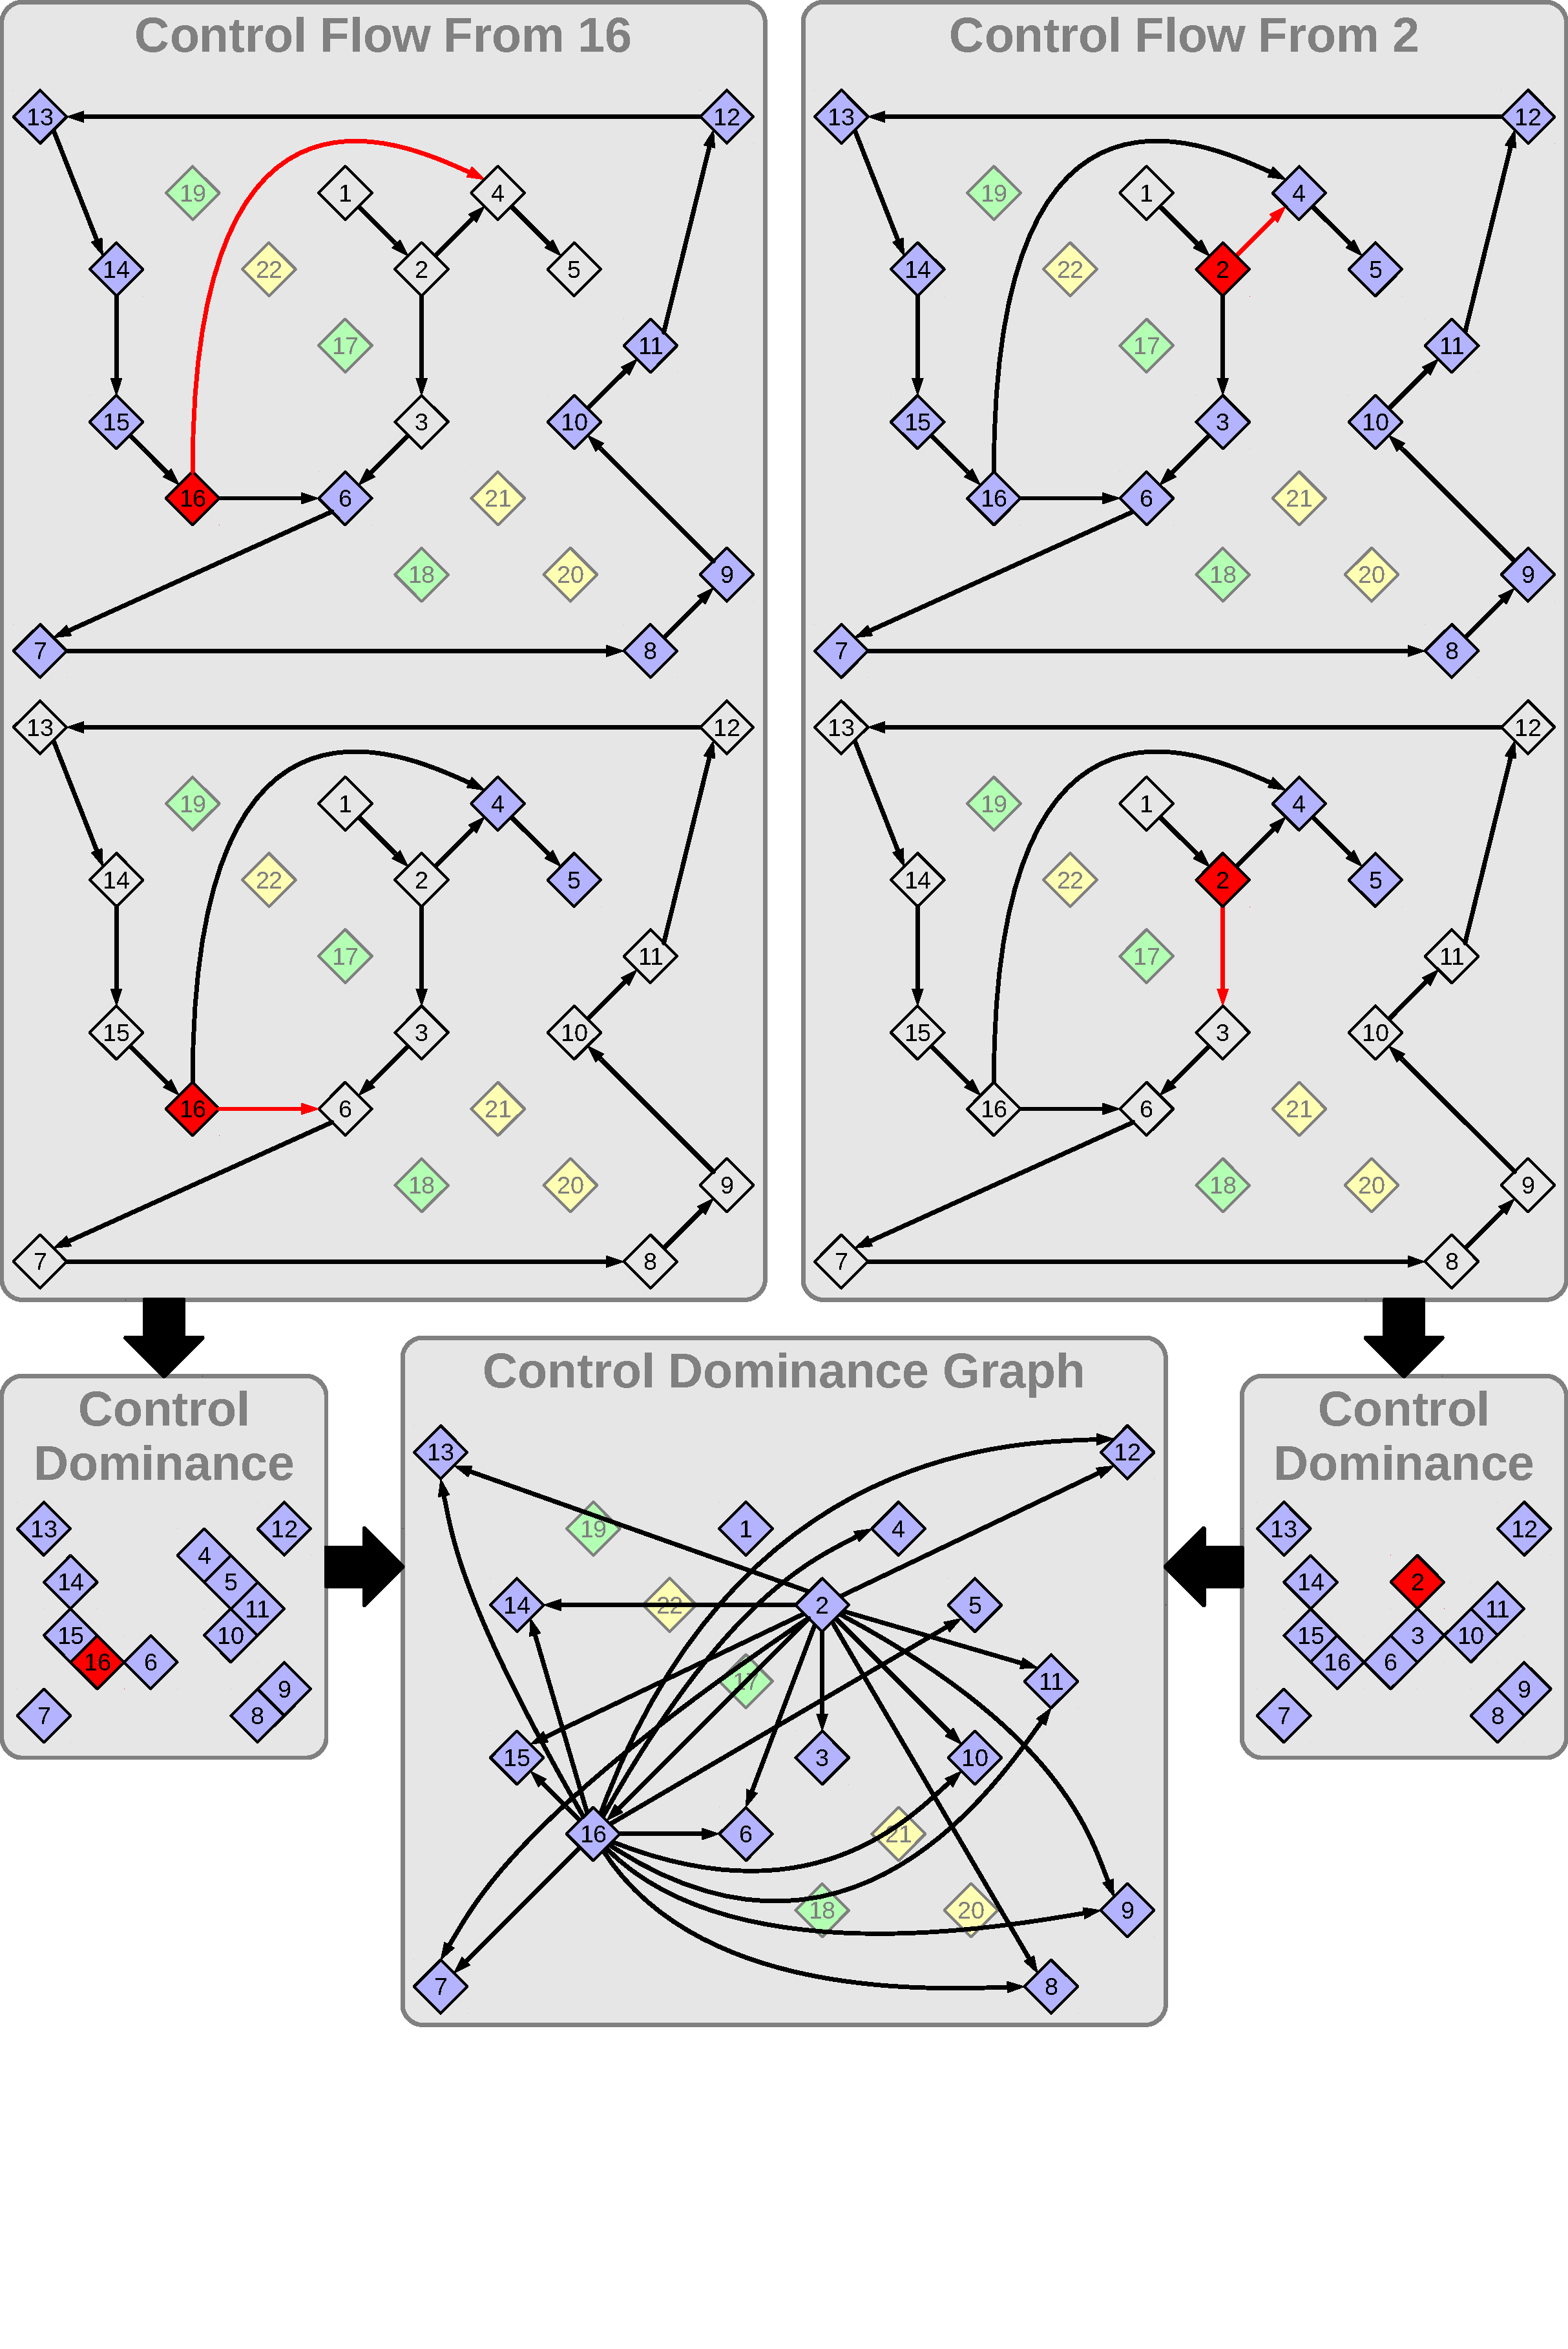
\includegraphics[width=\linewidth]{figures/schaubild2.pdf}
    \caption{Computation of the control dependence graph.}
    \label{fig:pdg}
\end{figure}

\subsection{Control Dependence Example}

    The control dependence graph is a function of the control flow graph, as is
    directly apparent from \autoref{def:cdg}.
    We can see how an example control dependence graph is computed in
    \autoref{fig:pdg}, from the control flow graph of the \texttt{dot} function
    in \autoref{fig:derivemaths}.
    From the definition it is immediately obvious that we need to only consider
    conditional branches as origins of control dependence.

    We can consider the two conditional branches $2$ and $16$ independently.
    On the right, we consider only $2$.
    We check the defining property: On the top of the figure, all the
    instructions that are not reachable from $2$ without the edge $(2,4)$ are in
    grey.
    Below this, all instructions not reachable from $2$ without $(2,3)$ are
    grey.
    We see that $4,5$ are always reachable and $1$ is never reachable, these are
    therefore not control dependent on $2$.
    All the other instructions are control dependent on $2$.

    Once we have computed this for all conditional branches, we take the union
    on graphs and get the complete control dependence graph of the function.
    Note what this graph represents:
    Once the loop in the function has been unrolled, it contains a conditional
    and a loop.
    Eveything within the body of the conditional is control dependent on $2$.
    Everythig within the loop as well as everything afterwards is control
    dependent on $16$.

\subsection{Phi Dependence Graph}

    Phi nodes are fundamental in single static assignment form and need special
    care.
    The value that a phi node takes depends on from where a phi node was
    reached.
    We need to encapsulate this in a graph.

    \begin{definition}{Phi Dependence Graph}{def:pog}
        Let $p$ a phi node and $c$ a conditional branch instruction.
        We say that the outcome of $p$ depends on $c$ if there is a branch
        instruction $b$ that reaches $p$ such that $b$ is control dependent on
        $c$.

        This defines the {\em phi dependence graph} $\Phi DG_\mathcal{F}$.
    \end{definition}

\subsection{Program Dependence Graph}

    After the control flow, data flow and control dependence graph, we lastly
    introduce the {\em program dependence graph}.
    It is the most exhaustive tool that we have to describe how values depend on
    each other.

    \begin{definition}{Program Dependence Graph}{def:pdg}
        The {\em program dependence graph} is defined as the union of data flow
        and control dependence graphs.
        \begin{align*}
            PDG_\mathcal{F}:=DFG_\mathcal{F}^*\cup CDG_\mathcal{F}^*\cup\Phi DG_\mathcal{F}\text{.}
        \end{align*}
    \end{definition}

    With the program dependence graph, we can now define subsections of the
    program that are self-contained and can be separated into their own
    function.
    This works even if they contain complicated control flow.
    Firstly, we need a definition of an interface.

    \begin{definition}{Interface}{def:interface}
        Let $a\in CFG_\mathcal{F}^*$ and $b_1,\dots,b_n\in DFG_\mathcal{F}^*$.
        Furthermore let $A\subset\mathbb{N}$ a set of instructions.

        We say that $(b_1,\dots,b_n)$ is an interface to $A$ if it is a cut
        between $o$ and $A$ in $PDG_\mathcal{F}$ for any of the following $o$:
        \begin{itemize}
            \item $o$ is a paramter
            \item $o$ is impure
        \end{itemize}
    \end{definition}


\newpage
\subsection{Interface Example}

    We will now consider a non-trivial example.
    Consider this snppet of C code, implementing a function that performs a
    simple square root approximation on each element in an array of double
    precision floating point values.

\begin{figure}[h]
\begin{lstlisting}[language=C]
void map_sqrt(size_t length, double* array)
{
    for(int i = 0; i < length; i++)
    {
        double root = 1.0;
        for(int i = 0; i < 10; i++)
            root = 0.5*(root+array[i]/root);

        array[i] = root;
    }
}
\end{lstlisting}
\caption{{\bf map$\circ$sqrt}: Apply an appriximate sqare root function to each
         element in a vector.}
\end{figure}

    Coneptually, we should be able to disentangle the square root function from
    the control flow of the outer loop.
    This is possible with the preceeding definition of {\em interfaces}.


\newpage
In single static assignment form, this code looks as follows:

\begin{lstlisting}[language=LLVM]
define void @map_sqrt(i64, double*) {
  %3 = icmp eq i64 %0, 0
  br i1 %3, label %5, label %4

; <label>:4:
  br label %6

; <label>:5:
  ret void

; <label>:6:
  %7 = phi i64 [ %10, %8 ], [ 0, %4 ]
  br label %12

; <label>:8:
  %9 = getelementptr double, double* %1, i64 %7
  store double %19, double* %9
  %10 = add nuw i64 %7, 1
  %11 = icmp eq i64 %10, %0
  br i1 %11, label %5, label %6

; <label>:12:
  %13 = phi i64 [ 0, %6 ], [ %20, %12 ]
  %14 = phi double [ 1.0, %6 ], [ %19, %12 ]
  %15 = getelementptr inbounds double, double* %1, i64 %13
  %16 = load double, double* %15
  %17 = fdiv double %16, %14
  %18 = fadd double %14, %17
  %19 = fmul double %18, 5.0
  %20 = add nuw nsw i64 %13, 1
  %21 = icmp eq i64 %20, 10
  br i1 %21, label %8, label %12
}
\end{lstlisting}

    In this example, the set $\{\%9\}$ is an interface to $\{(\%19,\%store)\}$.

\section{Formulating Constraint Problems}

    We will now use these mathematical background deliberations to derive
    constraint programming on top of LLVM code.

    Consider the following definitions of simple binary predicates:

    \begin{align*}
     is\_branch\_inst(\mathcal F, n):= (n,\text{\bf br})\in T_\mathcal{F}\\
     is\_control\_edge(\mathcal F, n, m):= (n,m)\in CFG_\mathcal{F}^*\\
     is\_control\_dom(\mathcal F, n, m):= \\
    \end{align*}

    We can then use these predicates to define more complex constructs, such as
    single entry, single exit (SESE) regions.

    \begin{definition}{}{}{}
        A single entry single exit region is a tuple $a,b,c,d\in\mathcal N$ such
        that the following properties hold:
        \begin{align*}
            is\_control\_edge(\mathcal{F},a,b)\\
            is\_control\_edge(\mathcal{F},c,d)\\
            is\_control\_dom(\mathcal{F},c,d)\\
            is\_control\_postdom(\mathcal{F},d,c)\\
        \end{align*}
    \end{definition}

    


\chapter{CAnDL: A Constraint Programming Language for SSA Code}

    Optimizing compilers require sophisticated program analysis and
    transformations to exploit modern hardware.
    Implementing the appropriate analysis for a compiler optimization is a time
    consuming activity.
    For example, in LLVM, tens of thousands of lines of code are required to
    detect appropriate places to apply peephole optimizations.
    It is a barrier to the rapid prototyping and evaluation of new
    optimizations.

    In this chapter, we develop the Compiler Analysis Description Language
    (CAnDL), a domain specific language for compiler analysis.
    Based on the constraint programming methodology that we established
    previously, CAnDL provides a convenient mechanism for programmers to 
    analyse LLVM's intermediate representation.
    It enables a workflow, where the compiler developer writes CAnDL programs,
    which is then compiled by the CAnDL compiler into a C++ LLVM pass.
    This provides a uniform manner in which to describe compiler analysis and
    can be applied to a range of compiler analysis problems, reducing code
    length and complexity.

    We implemented and evaluated CAnDL on a number of real world use cases:
    eliminating redundant operations; graphics code optimization; identifying
    static control flow regions.
    In all cases were we able to express the analysis more briefly than
    competing approaches.

\section{Introduction}

    Compilers are complex pieces of software responsible for the generation of
    efficient code. 
    This requires the careful application of a variety of optimizations. 
    Most optimizations can be split in two parts: analysis and transformation.
    The analysis is required to check for applicability and legality and often
    contains most of the complexity.
    For example, simple peephole optimizations in the LLVM {\tt instcombine}
    pass contain approximately 30000 lines of complex C++ code, despite the
    transformations being simple.

    This complexity is an impediment to the implementation of new compiler
    passes, preventing the rapid prototyping of new ideas.
    Ideally, we would like a simpler way of describing such analysis that
    reduces boiler-plate code and opens the way for new compiler optimization
    innovation.

    In this chapter we present CAnDL, a domain specific language for compiler
    analysis.
    It is a constraint programming language that operates on LLVM’s SSA-based
    IR.
    Instead of writing compiler analysis  code inside the main codebase of the
    compiler infrastructure, it enables compiler writers to specify optimization
    functionality external to LLVM.
    The CAnDL compiler generates a C++ function that is linked in and acts as an
    LLVM pass.
    The formulation of optimizing transformations in CAnDL is faster, simpler
    and less error prone than writing them in C++.
    It has a strong emphasis on modularity, which enables debugging and the
    formulation of highly readable code.

    We focus on programmer productivity and do not investigate formal methods
    for proving the correctness of optimization passes in this paper.
    However, previous work such as \cite{Lopes:2015:PCP:2737924.2737965}
    suggests that CAnDL would also be also suitable for automatic verification.

    We demonstrate the usefulness and generality of CAnDL via a number of use
    cases from different domains, including: standard LLVM optimization passes,
    custom optimizations for graphics shader programs and the detection of
    static control-flow regions for polyhedral program transformation.

    The core contributions of this papers are:
    \begin{itemize}
    \item The specification of a domain specific language for writing compiler
          analysis.\\[-0.9em]
    \item The implementation of the language inside of LLVM.\\[-0.9em]
    \item The evaluation of the approach on different compiler analysis case
          studies.
    \end{itemize}

\begin{figure*}[t]
    \begin{minipage}[t]{17.5cm}
\centering
\begin{minipage}[t]{6.422cm}
\centering
{\bf(a)} CAnDL program:
\begin{lstlisting}[language=CAnDL,basicstyle=\linespread{1.5565}\scriptsize\ttfamily]
Constraint SqrtOfSquare
( opcode{sqrt_call} = call
@∧@ {sqrt_call}.args[0]  = {sqrt_fn}
@∧@ function_name{sqrt_fn} = sqrt
@∧@ {sqrt_call}.args[1]  = {square}
@∧@ opcode{square} = fmul
@∧@ {square}.args[0] = {a}
@∧@ {square}.args[1] = {a})
End
\end{lstlisting}
\end{minipage}
\hfill
\begin{minipage}[t]{11cm}
\centering
\begin{minipage}[t]{11cm}
\centering
{\bf(b)} C program code:
\begin{lstlisting}
double example(double a, double b) { return sqrt(a*a) + sqrt(b*b); }
\end{lstlisting}
\end{minipage}
\begin{minipage}[t]{4.785cm}
\centering
{\bf(c)} Resulting LLVM IR:
\begin{lstlisting}[escapeinside={(*}{*)},language={LLVM}]
define double @example(    
 double %0,                
 double %1) {              
 %3 = fmul double %0, %0   
 %4 = call double @sqrt(%3)
 %5 = fmul double %1, %1   
 %6 = call double @sqrt(%5)
 %7 = fadd double %4, %6   
 ret double %7 }
declare double @sqrt(double)      
\end{lstlisting}
\end{minipage}
\hfill
\begin{minipage}[t]{3.03cm}
\centering
{\bf(d)} First solution:
\begin{lstlisting}[escapeinside={(*}{*)},language={LLVM},numbers=none]

a = %0

square = %3
sqrt_call = %4 




sqrt_fn = @sqrt
\end{lstlisting}
\end{minipage}
\hfill
\begin{minipage}[t]{3.03cm}
\centering
{\bf(e)} Second solution:
\begin{lstlisting}[escapeinside={(*}{*)},language={LLVM},numbers=none]


a = %1


square = %5
sqrt_call = %6


sqrt_fn = @sqrt
\end{lstlisting}
\end{minipage}
\end{minipage}
\end{minipage}

\begin{minipage}[t]{17.5cm}
\centering
\begin{minipage}[t]{9.743cm}
\centering
{\bf(f)} C++ transformation code:
\begin{lstlisting}
void transform(map<string,Value*> solution, Function* abs) {
    ReplaceInstWithInst(
       dyn_cast<Instruction>(solution["sqrt_call"]),
       CallInst::Create(abs, {solution["a"]}));
}
\end{lstlisting}
\end{minipage}
\hfill
\begin{minipage}[t]{7.652cm}
\centering
{\bf(g)} Transformed LLVM IR after DCE:
\begin{lstlisting}[escapeinside={(*}{*)},language={LLVM}]
define double @example(double %0, double %1) {              
 %3 = call double @abs(double %0) 
 %4 = call double @abs(double %1)
 %5 = fadd double %3, %4   
 ret double %5 }
\end{lstlisting}
\end{minipage}
\end{minipage}
%Detected optimization opportunities:
%\begin{lstlisting}[escapeinside={(*}{*)},language={}]
%{ "sqrt_call" : %4,
%  "sqrt_func" : @sqrt,
%  "square" :   %3,
%  "a" :        %0 },
%{ "sqrt_call" : %6,
%  "sqrt_func" : @sqrt,
%  "square" :   %5,
%  "a" :        %1 }
%\end{lstlisting}
%Optimized LLVM IR:
%\begin{lstlisting}[escapeinside={(*}{*)},language={LLVM}]
%define double example(double %0, double %1) {
%  %3 = call double @fabs(double %0)
%  %4 = call double @fabs(double %1)
%  %5 = fadd double %3, %4
%  ret double %5
%}
%\end{lstlisting}
\vspace{-0.3cm}
\caption{Demonstration of a simple CAnDL program}
\label{fig:firstexample}
    \label{fig:firstexample}
\end{figure*}

\section{Example}

    As a motivating example, assume that we want to use the algebraic property
    of the square root in \autoref{fig:root} to perform a floating point
    optimization (assuming the fast-math flag).
    \begin{align}
    \label{fig:root}
    \forall a\in \mathbb{R}\colon\ \sqrt{a*a}=|a|
    \end{align}

    In order to apply this transformation, the compiler must detect occurrences
    of $\sqrt{a*a}$ in the IR code and replace them with a call to the
    \texttt{abs} function.
    The generation of the new function call is trivial, but the detection of
    even a simple pattern like $\sqrt{a*a}$ requires some care when implementing
    it manually in a complex code base such as LLVM.

    The current approach would be to implement it as part of the
    \texttt{instcombine} pass, which already extends to almost 30000 lines of
    C++ code.
    This code makes heavy use of raw pointers and dynamic type casts.
    This is an impediment to compiler development and as previous work has shown
    \cite{Yang:2011:FUB:1993316.1993532,Menendez:2017:ADP:3062341.3062372}, it
    inevitably leads to buggy code.

    \autoref{fig:firstexample} shows how this optimization can be implemented
    with CAnDL.
    In (a), we can see the CAnDL program for the analysis. 
    It states that a section of LLVM code is eligible for optimization if seven
    individual constraints simultaneously hold on the values
    \texttt{sqrt\_call}, \texttt{sqrt\_func}, \texttt{square}, \texttt{a}.
    The lines 2-8 each stipulate one of these constrains and they are joined
    together with the logical conjunction operator. 

    This CAnDL program can be compiled with our CAnDL compiler into LLVM
    analysis functionality and (b)-(f) show the results of running it on an
    example program.
    In (b), we can see a simple C program that calls the \texttt{sqrt} function
    twice with squares of floating point values. 
    Below this, in (c), we see LLVM IR that is generated from the C code.
    I involves two \texttt{fmul} instructions to generate the squares via a
    floating point multiplication and two calls to the \texttt{sqrt} function
    with the respective result. 

    Note that for each application of the \texttt{sqrt} function there is a call
    instruction {\it e.g.} {\tt \%4 = call \dots} and the actual \texttt{sqrt}
    function is the first argument of these call instructions.

    The CAnDL program detects two opportunities to apply the transformation,
    shown in (d) and (e).
    Each of the two solutions assigns values from within the IR code to each of
    the variables in the CAnDL program such that all constraints are fulfilled.
    Let us look in detail at the first solution.
    \begin{itemize}
    \item \texttt{\%4} is assigned to \texttt{sqrt\_call}. It is a function call
          (Line 2 of CAnDL program) to the \texttt{sqrt} function (Lines 3 and 4
          of CAnDL program).
    \item \texttt{@sqrt} is assigned to \texttt{sqrt\_func}. It is the standard
          library function \texttt{sqrt} (Line 4 of CAnDL program). 
    \item \texttt{\%3} is assigned to \texttt{square}. It is the second argument
          of \texttt{\%4} (\texttt{sqrt\_call}) and it is an \texttt{fmul}
          instruction (Lines 5 and 6 of CAnDL program).
    \item \texttt{\%0} is assigned to \texttt{a}. It is the first and second
          argument of \texttt{\%3} (\texttt{square}) (lines 7-8 of CAnDL
          program).
    \end{itemize}

    With the analysis functionality provided by CAnDL, the transformation is now
    simple.
    In \autoref{fig:firstexample} (f) we can see how the result of the analysis
    in the form of a C++ dictionary {\it std::map<std::string,llvm::Value*>}
    contains all the required information.
    A new function call to {\tt abs} is generated with the solution for {\tt a}
    as the only argument.
    This instruction then replaces the original call instruction that was
    captured in {\tt sqrt\_call}.
    After standard dead code elimination this results in the optimized code
    shown in (g).


    Although this is a small example, it illustrates the main steps in our
    scheme.
    In practice, however, we wish to detect more complex code using constraints
    on control and data flow structure.
    In the next section we introduce a powerful description language that is
    capable of defining a wide class of analysis.

\section{Language Specification}

    The Compiler Analysis Description Language (CAnDL) is a domain specific
    constraint programming language for the specification of compiler analysis
    passes. 
    Individual CAnDL programs define computational structures to be exploited by
    optimizing code transformations.
    These structures are specified as constraints on single static assignment
    (SSA) form representations of programs.

    Structures can scale from simple instruction patterns that are suited for
    peephole optimizations over basic control flow structures such as loops to
    complex algorithmic concepts such as stencil codes with arbitrary kernel
    functions or code regions suitable for polyhedral analysis.

    The basic building blocks of CAnDL programs are well known compiler analysis
    tools, such as constraints on data and control flow, data types and
    instruction opcodes.
    On top of these low level constraints, CAnDL employs powerful mechanisms for
    modularity and encapsulation that allow the construction of complex
    programs.

\subsection{High Level Structure of CAnDL Programs}

    An individual CAnDL program contains a set of constraint formulas that are
    bound to identifiers.
    As we already saw in \autoref{fig:firstexample} (a), the syntax for this is
    as follows:
    \begin{align*}
        \text{\bf Constraint}\ \left<\text{\bf s}\right>\ \text{\it formula}\ \text{\bf End}
    \end{align*}
    For the description of CAnDL syntax we use these notational conventions:
    terminal symbols are {\bf bold}, non-terminals are {\it italic},
    $\left<\text{\bf s}\right>$ is an identifier (alphanumeric string) and
    $\left<\text{\bf n}\right>$ is an integer literal.

    We already saw in \autoref{fig:firstexample} (a) that logical conjunctions
    can be used to combine {\it formula}s.
    More generally, a {\it formula} can be any of the following:
    \begin{align*}
        &\text{\it atomic}\mid\text{\it conjunction}\mid \text{\it disjunction}\\
        \mid{}&{}\text{\it foreach}\mid \text{\it forany}\mid\text{\it include}\mid\text{\it collect}
    \end{align*}
    The basis of every CAnDL program are {\it atomic} constraints.
    For example in \autoref{fig:firstexample} (a), lines 2-8 each specify
    individual atomic constraints.
    Atomic constraints are bound together by logical connectives $\land$ and
    $\lor$ ({\it conjunction} and {\it disjunction}) and other higher level
    constructs.
    These include two kinds of loop structures ({\it foreach}, {\it forany}), as
    well as a system for modularity (\texttt{include}).
    Lastly, the {\it collect} construct allows for the formulation of more
    complex constraints that require the $\forall$ quantifier.

\subsection{Atomic Constraints}

    The first type of constraint is an {\it atomic} constraint based on
    {\it variable}s.
    {\it Variable}s in CAnDL correspond to instructions and values in LLVM IR. 
    Given some IR code, all occurring values can be assigned to the
    {\it variable}s of a given constraint formula.
    This includes instructions, globals, constants and function parameters.
    Syntactically, a variable is simply an identifier in curly brackets.

    CAnDL uses the following atomic constraints:
    \begin{align*}
        \text{\bf data\_type}\ \text{\it variable}\ &\text{\bf =}\ \text{\bf int}\\
        \text{\bf data\_type}\ \text{\it variable}\ &\text{\bf =}\ \text{\bf float}
    \end{align*}
    This restricts the data type to integer or floating point.
    \begin{align*}
        \text{\bf ir\_type}\ \text{\it variable}\ &\text{\bf =}\ \text{\bf literal}\\
        \text{\bf ir\_type}\ \text{\it variable}\ &\text{\bf =}\ \text{\bf argument}\\
        \text{\bf ir\_type}\ \text{\it variable}\ &\text{\bf =}\ \text{\bf instruction}
    \end{align*}
    This restricts the type of IR node that is allowed to compile time constants, function arguments or instructions.
    \begin{align*}
        \text{\bf opcode}\ \text{\it variable}\ &\text{\bf =}\ \left<\text{\bf s}\right>
    \end{align*}
    This restricts the value instructions of the specified opcode.
    \begin{align*}
        \text{\bf function\_name}\ \text{\it variable}\ \text{\bf =}\ \left<\text{\bf s}\right>
    \end{align*}
    This restricts the variable to be a specified standard function (i.e.\ the {\tt sqrt} function).
    \begin{align*}
        \text{variable}\ &\text{\bf =}\ \text{variable}\\
        \text{variable}\ &\text{\bf !=}\ \text{variable}
    \end{align*}
    This enforces two variables to have the same/not the same value.
    This is a shallow comparison, i.e. it compares whether two variables represent the same IR node. 
    \begin{align*}
        \text{\bf control\_origin}&\ \text{\it variable}\\
        \text{\bf data\_origin}&\ \text{\it variable}
    \end{align*}
    The value is an origin of control (function entry) or data (function argument, {\tt load} instruction, inpure function call).
    \begin{align*}
        \text{\it variable}\text{\bf.arg[}\left<\text{\bf n}\right>{\bf]}\ &\text{\bf =}\ \text{\it variable}\\
        \text{\it variable}\ &\text{\bf $\in$}\ \text{\it variable}\text{\bf .args}
    \end{align*}
    There data flow from one value to the next.
    \begin{align*}
        \text{\it variable}\ \text{\bf ->}\ \text{\it variable}\ \Phi\ \text{\it variable}
    \end{align*}
    The left value has to reach the right value, which is a phi node, via the middle value, which is a jump instruction.
    \begin{align*}
        \text{\bf domination(}\text{\it variable}\text{\bf,} \text{\it variable}\text{\bf)}&\\
        \text{\bf strict\_domination(}\text{\it variable}\text{\bf,} \text{\it variable}\text{\bf)}&
    \end{align*}
    Both values have to be instructions and the first dominates the second in the control flow graph.
    \begin{align*}
        \text{\bf calculated\_from(}\text{\it varlist}\text{\bf,}\text{\it varlist}\text{\bf,}\text{\it variable}\text{\bf)}
    \end{align*}
    {\it Varlist} is a set of one or multiple {\it variables}.
    Any path from one of the entries in the first {\it varlist} to the single
    {\it variable} argument has to pass through at least one of the entries in
    the second {\it varlist}.
    All paths in the union of the data flow and control dependence graph are
    considered.
    We will see later how this is useful to specify kernel functions for
    e.g.\ stencil calculations.

    There are some {\it atomic}s that we omit for space reasons.
    The set of {\it atomic}s that CAnDL supports is easily extensible.
    Possible additions include constraints on function attributes, value
    constraints on literals etc.

\subsection{Range Constraints}

    Building on top of the basic conjunction and disjunction constructs, there
    are range based versions that operate on arrays of variables.
    \begin{align*}
        \text{\it formula}\ &\text{\bf foreach}\ \left<\text{\bf s}\right>\ \text{\bf =}\ \text{\it index}\ \text{\bf ..}\ \text{\it index}\\
        \text{\it formula}\ &\text{\bf forany}\ \left<\text{\bf s}\right>\ \text{\bf =}\ \text{\it index}\ \text{\bf ..}\ \text{\it index}
    \end{align*}
    These constructs allow the repeated application of a formula according to
    some range of indices.
    This is demonstrated by \autoref{fig:forall}, which shows two equivalent
    CAnDL programs, one formulated with \texttt{foreach} and one without.
    In both cases, the program specifies an array of five variables with data
    flow from each element to the next.
    We can see how the \texttt{foreach} loop can be expanded similar to loop
    unrolling.

\begin{figure}[ht]
\begin{lstlisting}[language=CAnDL]
Constraint ValueChain
 {element[i] ([$\tt \in$]) {element[i+1]}.args foreach i=0..4
End
\end{lstlisting}
\begin{lstlisting}[language=CAnDL]
Constraint ValueChain
( {element[0]} ([$\tt \in$]) {element[1]}.args
([$\tt \land$]) {element[1]} ([$\tt \in$]) {element[2]}.args
([$\tt \land$]) {element[2]} ([$\tt \in$]) {element[3]}.args
([$\tt \land$]) {element[3]} ([$\tt \in$]) {element[4]}.args)
End
\end{lstlisting}
\vspace{-0.3cm}
\caption{Expansion of range constraints in CAnDL}
\label{fig:forall}
\end{figure}

\subsubsection{Modularity}
    \label{sec:modularity}

    Modularity is central to the CAnDL programming language, and it is achieved
    using the {\it include} construct.
    \begin{align*}
        \text{\bf include}\ &\left<\text{\bf s}\right>\\
                            &[\text{\bf (}\text{\it variable}\ \text{\bf ->}\ \text{\it variable}\ \{\text{\bf ,}\ \text{\it variable}\ \text{\bf ->}\ \text{\it variable}\}\text{\bf )}]\\
                            &[\text{\bf @}\ \text{\it variable}]
    \end{align*}
    Note that the syntax in square brackets is optional and the syntax in curly
    brackets can be repeated.
    The basic version of \texttt{\it include}, without the optional structures,
    is simple.
    It copies the {\it formula} that corresponds to the identifier verbatim into
    another {\it formula}.
    If $[\text{\bf @}\ \text{\it variable}]$ is specified, then all the variable
    names of the inserted constraint formula are prefixed with the given
    variable name, separated with a dot.
    The other optional syntax is used to rename individual {\it variable}s in
    the included {\it formula}.

    \autoref{fig:inheritsandrenameandrebase} illustrates this with two
    equivalent programs.
    Both programs specify an addition of four values, first adding pairwise and
    then adding the intermediate results.
    We can see in the first listing that a {\it formula} for the addition of two
    values is bound to the name {\tt Sum}.
    This is then included three times in another {\it formula} names
    {\tt SumOfSums}.
    Using the optional grammatical constructs, the formula operates on a
    different set of {\it variable}s each time such that the third addition
    takes the results of the previous two as input.

\begin{figure}[ht]
\begin{lstlisting}[language=CAnDL]
Constraint Sum
( opcode{out} = add
([$\tt \land$]) {out}.args[0] = {in1}
([$\tt \land$]) {out}.args[1] = {in2})
End
Constraint SumOfSums
( include Sum@{sum1}
([$\tt \land$]) include Sum@{sum2}
([$\tt \land$]) include Sum({sum1.out}->{in1},{sum2.out}->{in2}))
End
\end{lstlisting}
\begin{lstlisting}[language=CAnDL]
Constraint SumOfSums
( opcode{sum1.out} = add
([$\tt \land$]) {sum1.out}.args[0] = {sum1.in1}
([$\tt \land$]) {sum1.out}.args[1] = {sum1.in2}
([$\tt \land$]) opcode{sum2.out} = add
([$\tt \land$]) {sum2.out}.args[0] = {sum2.in1}
([$\tt \land$]) {sum2.out}.args[1] = {sum2.in2}
([$\tt \land$]) opcode{out} = add
([$\tt \land$]) {out}.args[0] = {sum1.out}
([$\tt \land$]) {out}.args[1] = {sum2.out})
End
\end{lstlisting}
\vspace{-0.3cm}
\caption{Expansion of Inheritance in CAnDL}
\label{fig:inheritsandrenameandrebase}
\end{figure}

\subsubsection{Collect}

    The \text{\it collect} construct is used to capture all possible solutions
    of a given formula.
    It is used to implement constraints that require the logical $\forall$
    quantifier.
    For example, it can be used to guarantee that all memory accesses in a loop
    use affine index computations.
    The grammar is simple but the semantics require some elaboration.
    \begin{align*}
        \text{\bf collect}\ \left<\text{\bf s}\right>\ \text{\it index}\ \text{\it formula}
    \end{align*}
    In \autoref{fig:simplecollect}, the variables \texttt{arg[0],\dots,arg[N-1]}
    are constraint to contain all data dependences of \texttt{ins}.
    The first argument of \text{\it collect} specifies the name of an index
    variable that is used to detect which variables belong to the collected set.
    In this example we want all solutions of \texttt{arg[i]} for a given value
    of \texttt{ins}.
    The second argument gives an upper bound to the amount of collected
    variables, in this case we leave it unspecified by using the symbol
    \texttt{N}.

\begin{figure}[h]
\begin{lstlisting}[language=CAnDL]
Constraint CollectArguments
( ir_type{ins} = instruction
([$\tt \land$]) collect i N ({arg[i]} ([$\tt \in$]) {ins}.args))
End
\end{lstlisting}
\vspace{-0.3cm}
\caption{Simple collect example in CAnDL}
\label{fig:simplecollect}
\end{figure}

    We can now extend this example to show how {\it collect} can be used to
    implement quantifiers.
    Consider that we want to detect instructions with only floating point data
    dependences.
    Formulating this involves the $\forall$ quantifier, as it is equivalent to
    the following equation.
    \begin{align}
        \forall v\colon\ v\in I.\text{args}\implies\text{data\_type}(v)=\text{float}
    \label{fig:implication}
    \end{align}
    We can rewrite this to an equivalent formulation on sets.
    \begin{align*}
        S_1:= \{v\mid v\in I.\text{args}\}\subset S_2:={}\{v\mid\text{data\_type}(v)=\text{float}\}
    \end{align*}
    Now we can apply the following equivalences:
    \begin{align*}
        &S_1\subset S_2\Leftrightarrow{}S_1 = S_1\cap S_2\\
        \Leftrightarrow{}&\exists S\colon S=S_1\land S=S_1\cap S_2
    \end{align*}
    This means that if we constraint a set $S$ to be equal to both $S_1$ and
    $S_1\cap S_2$ at the same time, the constraints are satisfiable if and only
    if the implication in \autoref{fig:implication} holds.

    This condition can be expressed in CAnDL, as is shown in
    \autoref{fig:collectexample}.
    With the first {\it collect} statement in line 3, we constrain the set
    \texttt{arg} to be equal to $S_1$ and with the second one in lines 4-5 we
    constrain it to be $S_1\cap S_2$ as well.
    Note that we were from the onset only interested in the values that qualify
    for \texttt{ins}.
    The set \texttt{arg} was only introduced to further constraint \texttt{ins},
    not because we actually wanted to know the values that it contains.

\begin{figure}[h]
\begin{lstlisting}[language=CAnDL]
Constraint FloatingPointInstruction
( ir_type{ins} = instruction
([$\tt \land$]) collect i N ( {ins} ([$\tt \in$]) {arg[i]}.args)
([$\tt \land$]) collect i N ( {ins} ([$\tt \in$]) {arg[i]}.args
              ([$\tt \land$]) data_type{arg[i]} = float))
End
\end{lstlisting}
\vspace{-0.3cm}
\caption{Collect Example in CAnDL}
\label{fig:collectexample}
\end{figure}

    The exact same approach can be used to e.g. restrict all array accesses in a
    loop to be affine in the loop iterators.
    This can be achieved by first {\it collect}ing all memory accesses
    (i.e.\ all \texttt{load} and \texttt{store} instrutions) and then using
    another {\it collect} statement to stipulate affine calculations for the
    indices.

\subsection{Expressing Larger Structures}

    The modularity of CAnDL allows the creation of a library of building blocks
    that are shared by multiple CAnDL programs.
    We will now give an overview about how these can be defined with CAnDL.

    Important building blocks include control flow structures such as single
    entry single exit regions and loops.
    These are standard in compiler analysis and the implementation in CAnDL is
    straightforward.
    A for loop involves a comparison of the loop iterator with the end of the
    iteration space.
    In order to be valid, this value has to be determined before the loop is
    entered, it isn't allowed to change from loop iteration to iteration.
    This leaves it to be either a function argument, an actual constant or an
    instruction that strictly dominates the loop entry.
    This is expressed in \autoref{fig:localconstant}.
    Note that this formula is to be included into larger CAnDL programs, as the
    \texttt{begin} variable is under specified otherwise.

\begin{figure}[h]
\begin{lstlisting}[language=CAnDL]
Constraint LocalConst
( ir_type{value} = literal
([$\tt \lor$]) ir_type{value} = argument
([$\tt \lor$]) strict_domination({value}, {begin}))
End
\end{lstlisting}
\vspace{-0.3cm}
\caption{LocalConst in CAnDL}
\label{fig:localconstant}
\end{figure}

    Another class of important building blocks are different categories of
    memory access.
    These form a hierarchy of restrictiveness and include multidimensional array
    access and array access that is affine in some loop iterators.
    LLVM strictly separates memory access from pointer computations, which means
    that CAnDL only has to concern itself with pointer computations here.
    In general it is required that the base pointer is \texttt{LocalConst} in
    order to avoid pointer chases.
    The index computation can then be described using the data flow and
    instruction opcode restrictions.

    To enable the capture of higher order functions such as stencils or
    reduction operations, we need to handle arbitrary kernel functions.
    Kernel functions are sections of code that are side-effect free and
    can be separated out. Identifying side-effect free code is useful in
    many types of compiler optimization.  It can be expressed in CAnDL, as
    shown in \autoref{fig:kernel}.

\begin{figure}[h]
\begin{lstlisting}[language=CAnDL]
Constraint KernelFunction
( collect i N
([$\tt \land$]) ( include LocalConst({outer}->{begin}*@*{closure[i]}
  ([$\tt \land$]) ir_type{closure[i].value} != literal
  ([$\tt \land$]) {closure[i].use} ([$\tt \in$]) {closure[i].value}.args
  ([$\tt \land$]) domination({inner}, {closure[i].use}))
([$\tt \land$]) collect i N data_origin{tainted1[i]}
([$\tt \land$]) collect i N
([$\tt \land$]) ( domination({outer}, {tainted2[i]})
  ([$\tt \land$]) strict_domination({tainted2[i]}, {inner}))
([$\tt \land$]) calculated_from(
   {tainted1[0..N],tainted2[0..N]},
   {origin[0..N],closure[0..N].value,input[0..N]},
   {output}))
End
\end{lstlisting}
\vspace{-0.3cm}
\caption{CAnDL Formulation of Kernel Functions}
\label{fig:kernel}
\end{figure}

    Essentially, this set of contraints captures the computation of a
    single \texttt{output} value from a set of specified \texttt{input}
    values as well as a set of automatically captured \texttt{closure}
    variables.  The computation for \texttt{output} should be such that it
    can be replaced with a function call that is free of side effects and
    takes only the \texttt{input} and \texttt{closure} variables as
    arguments.

    In addition to these variables, there are two non-obvious additional
    variables involved: \texttt{outer} and \texttt{inner}.
    These set boundaries in the control flow as follows: Closure values have to
    be computed before \texttt{outer} and the computation that results in outer
    is performed after \texttt{inner}.
    Usually these will be derived from loops nests, where \texttt{outer} is the
    entry to the outermost loop and \texttt{inner} is the entry to the innermost
    loop.
    The actual core constraint is then a generalized dominance relationship in
    the program dependence graph.

    The use of the sets \texttt{tainted1} and \texttt{tainted2} makes sure that
    no impure functions are used in computing \texttt{output} and the entire
    computation is performed after \texttt{inner} (ruling out e.g.\ loop carried
    variabls from outer loops).

\section{Implementation}

    CAnDL interacts with the LLVM framework, as shown in \autoref{fig:build2}.
    CAnDL programs are read by the CAnDL compiler, which then generates C++
    source code to implement the specified LLVM analysis functionality.
    This code depends on a generic backtracking solver, which is incorporated
    into the main LLVM code base. 
    We will see in the evaluation section this this solver adds little
    compile-time overhead in practice.
    The generated code is compiled and linked together with the existing LLVM
    libraries to make LLVM optimization passes available in the clang compiler.

    The generated analysis passes use the solver to search for the specified
    computational structures and output the found instances into report files,
    as well as making them available to ensuing transformation passes.

\begin{figure}[ht]
\centering
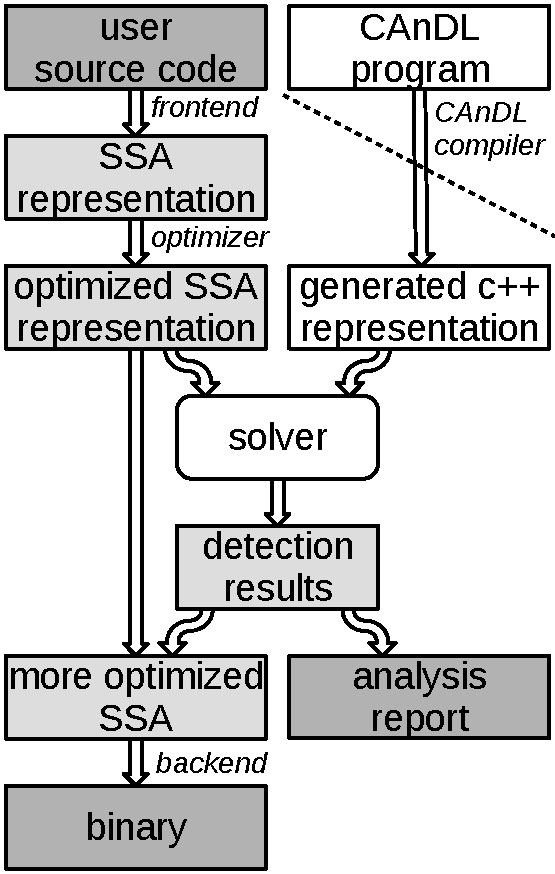
\includegraphics[width=0.29\textwidth]{figures/compilerFlow2.pdf}
\caption{CAnDL in the LLVM/clang build system}
\label{fig:build2}
\end{figure}

\subsection{The CAnDL Compiler}

\begin{figure}[t]
\centering
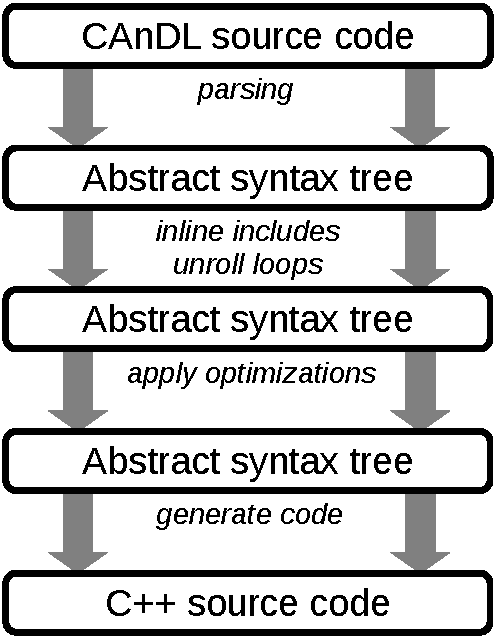
\includegraphics[width=0.29\textwidth]{figures/compilerFlow.pdf}
\caption{CAnDL compiler flow}
\label{fig:compilerflow}
\end{figure}

    The CAnDL compiler is responsible for generating C++ code from CAnDL
    programs.
    An overview of its  flow is shown in \autoref{fig:compilerflow}.
    The frontend reads in  CAnDL source code and builds an abstract syntax tree.
    This syntax tree is simplified in two steps to eliminate some of the higher
    order constructs of CAnDL.
    The \texttt{inheritance} clauses are replaced using standard function
    inlining after the contained variables have been transformed accordingly.
    Also, \texttt{foreach} and \texttt{forany} statements are lowered to
    conjunctions and disjunctions by duplicating the contained constraint code
    and then renaming the contained variable names appropriately for each
    iteration. This is equivalent to complete loop unrolling.
    From this point onwards, variable names are treated as flat strings.
    The remaining core language now consists only of atomics, conjunctions,
    disjunctions and collections.

    The CAnDL compiler applies a set of basic optimizations to speed up the
    solving process using the later generated C++ code.
    For example, nested conjunctions and disjunctions are flattened wherever
    possible.

    Finally, the compiler generates the C++ source code.
    This essentially involves constructing the constraint problem as a graph
    structure that is accessible to the solver.

\subsubsection{C++ Code Generation}

    We demonstrate the code generation process in \autoref{fig:codegen} with an
    example.
    Each of the atomic constraints results in a line of C++ code that constructs
    an object of a corresponding class:
    In this case, the three involved atomic constraints are implemented by
    \texttt{AddInstruction}, \texttt{FirstArgument} and \texttt{SecondArgument}.
    For constraints that involve more than one variable, these objects are
    instantiated as shared pointers.

    The compiler then generates similar objects for the more complex
    \texttt{conjunction}, \texttt{disjunction} and \texttt{collect} structures.
    In our example, this only affects the variable \texttt{addition}, which is
    part of a \texttt{conjunction} clause.
    This results in an additional object construction that instantiates the
    \texttt{And} class corresponding to the {\bf $\land$} operator in CAnDL.
    The \texttt{select} function is used here to specify which variable of a
    constraint is being operated on.
    In this case, \texttt{addition} is the second variable in lines 3-4 of the
    CAnDL program, so we use \texttt{select<1>}.

    Finally, the generated objects are inserted into a vector together with the
    corresponding variable names.
    This vector is then passed to the solver.

\begin{figure}[ht]
\centering
\begin{lstlisting}[language=CAnDL]
Constraint SimpleAddition
( opcode{addition} = add
([$\tt \land$]) {addition}.args[0] = {left}
([$\tt \land$]) {addition}.args[1] = {right})
End
\end{lstlisting}
\begin{lstlisting}[language=C++]
auto constr0 = AddInstruction(context);
auto constr1 = make_shared<FirstArgument>(context);
auto constr2 = make_shared<SecondArgument>(context);
auto constr3 = And(constr0, select<1>(constr1),
                            select<1>(constr2));

vector<pair<string,SolverAtomContainer>> result(3);
result.emplace_back("addition", constr3);
result.emplace_back("left", select<0>(constr1));
result.emplace_back("right", select<0>(constr2));
\end{lstlisting}
\vspace{-0.3cm}
\caption{C++ source code generation}
\label{fig:codegen}
\end{figure}

\subsection{The Solver}

    The solver takes  LLVM IR code and a graph representation of the constraint
    problem as constructed by the generated code.
    We saw in \autoref{fig:codegen} that this representation comes in the form
    of a vector of labeled instances of a class called
    \texttt{SolverAtomContainer}.
    This class wraps around the class \texttt{SolverAtom} that is defined in
    \autoref{lst:solveratom}.

\begin{figure}[ht]
\begin{lstlisting}
class SolverAtom {
public:
  virtual SkipResult skip_invalid(unsigned& c)const;

  virtual void begin();
  virtual void fixate(unsigned c);
  virtual void resume();
};
\end{lstlisting}
\vspace{-0.3cm}
\caption{The SolverAtom interface.}
\label{lst:solveratom}
\end{figure}

    The motivation for this interface is as follows:
    The solver operates on unsigned integers, using the \texttt{skip\_invalid}
    method to search for partial solutions.
    The corresponding LLVM values are numbered consecutively and the unsigned
    integers simply represent indices into that enumeration.
    When \texttt{skip\_invalid} returns \texttt{FAIL}, the solver backtracks.
    The other member functions \texttt{begin}, \texttt{fixate} and
    \texttt{resume} allow implementations of the \texttt{SolverAtom} interface
    to do bookkeeping.

    Pseudocode for the backtracking constraint solver is shown in
    \autoref{fig:solver}.
    The array of \texttt{SolverAtom}s is named \texttt{atom}, \texttt{solution}
    is an array of integers that is incrementally filled with a solution to the
    constraint problem.
    In line 3, we can see that the \texttt{skip\_invalid} method is used to find
    the next candidate solution for the \texttt{i}th element of the solution,
    taking into account all the previously established elements
    \texttt{solution[0..i-1]}.
    The candidate solution is directly stored in \texttt{solution[i]}, which is
    passed by reference as shown in \autoref{lst:solveratom}.
    If the step was successful, then the solver either returns the solution if
    it is complete or it moves on the the next element (line 11), otherwise it
    backtracks (line 16).
    The member function \texttt{fixate}, \texttt{begin} and \texttt{resume} are
    called appropriately in lines 6, 12 and 17.

\begin{figure}[t]
\begin{lstlisting}
i := 0
while i >= 0:
    result := atom[i].skip_invalid(solution[i])

    if result = SkipResult::PASS:
        atom[i].fixate(solution[i])

        if i+1 = N:
            return solution
        else:
            i := i+1
            solver_atom[i].begin()
            solution[i] := 0

    if result = SkipResult::FAIL:
        i := i-1
        atom[i]->resume()
        solution[i] := solution[i]+1
\end{lstlisting}
\vspace{-0.3cm}
\caption{Pseudocode of the backtracking solver}
\label{fig:solver}
\end{figure}

    We can see that the solver is generic and requires no knowledge of LLVM or
    the structure of variable names in CAnDL.
    Furthermore, the solver is unaware not only of the underlying LLVM structure
    and the corresponding atomic constraints, but also of the
    \texttt{conjunction}, \texttt{disjunction} and \texttt{collect} constructs.

    The complexity of the solving process lies almost entirely in the
    implementation of the \texttt{SolverAtom} interface for the different atomic
    constraints and their interactions.
    For simple constraints like the \textbf{is an add instruction} statement,
    this is straightforward and \texttt{skip\_invalid} only has to test whether
    the value at \mbox{index n} in the function is an add instruction or not.
    This can be implemented as shown in \autoref{lst:solveratomadd}.

\begin{figure}[ht]
\begin{lstlisting}
class AddInstruction : public SolverAtom {
public:
  AddInstruction(Context&) { ... }

  SkipResult skip_invalid(unsigned& c) const
  {
      if(c >= value_list->size())
        return SkipResult::FAIL;

      if(auto inst = dyn_cast<Instruction>
                       ((*value_list)[c]))
      {
        if(inst->getOpcode() == Instruction::Add)
          return SkipResult::PASS;
      }

      c=c+1;
      return SkipResult::CHANGE;
  }

  void begin() {}
  void fixate(unsigned c) {}
  void resume() {}

private:
  shared_ptr<vector<Value*>> value_list;
};
\end{lstlisting}
\vspace{-0.3cm}
\caption{SolverAtom for additions}
\label{lst:solveratomadd}
\end{figure}

\begin{figure*}[ht]
\centering
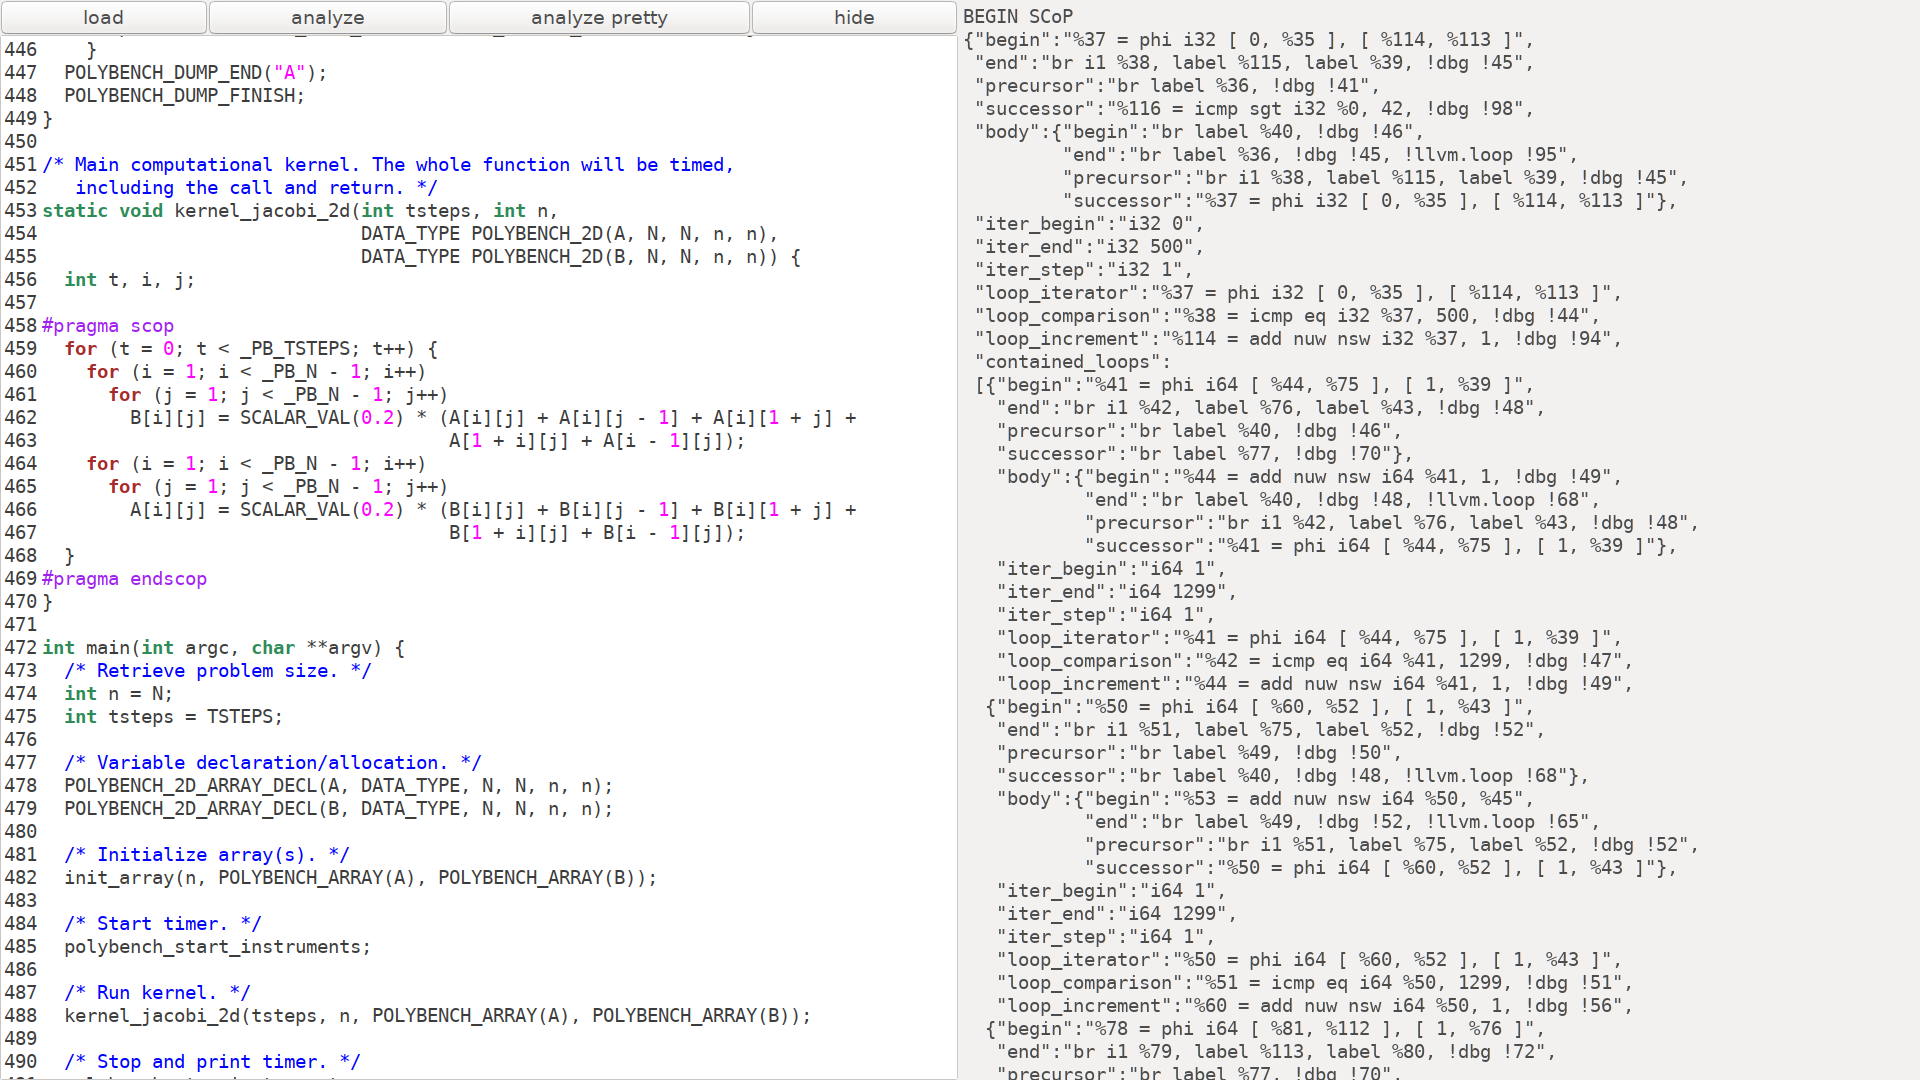
\includegraphics[width=0.9\textwidth]{figures/visual_gui2.png}
\caption{Interactive CAnDL test tool}
\medskip
\small
Left hand panel shows a SCoP in Polybench jacobi-2d, the right hand panel show the corresponding constraint solution
\label{fig:gui}
\end{figure*}

\subsection{Developer Tools}

    CAnDL makes writing compiler analysis passes easier, but reasoning about the
    semantics of compiler IR still remains difficult and the correctness of
    CAnDL programs can only be guaranteed with thorough testing.
    It is important to keep in mind that CAnDL is targeted at expert compiler
    developers.

    In order to make debugging of CAnDL programs more feasible, we developed
    supporting tools.
    Most importantly, this includes an interactive gui, where developers can
    test out corner cases of CAnDL programs to find false positives and false
    negatives.
    This gui is shown in \autoref{fig:gui}, the example is from one of the use
    cases presented in a \autoref{sec:casestudies}.

    In the left column, we can see part of a C program from the PolyBench
    benchmark suite, which implements a two-dimensional Jacobi stencil.
    The gui is configured to look for static control flow regions (SCoPs), as
    described later in one of the use cases.
    The user has clicked the ``analyze'' button, which triggered the analysis to
    run and prints the results in the right column.

    The solver found a SCoP in the IR code (corresponding to lines 459-468 of
    the C program).
    The text on the right shows the hierarchical structure of the solution, with
    IR values assigned to every variable.
    The corresponding C code entities can be recovered using the debug
    information that is contained in the generated LLVM IR code.
    By modifying the C code, the developer can now test the detection and
    e.g.\ verify that no SCoP is detected if irregular control flow is
    introduced.


    We evaluate the usefulness of CAnDL on three real life use cases.
    We first use it  for  simple peephole optimizations.
    We then apply CAnDL to graphics shader code optimization.
    Finally, we demonstrate the detection of static control flow parts (SCoPs)
    for polyhedral code analysis.
    Where possible, we compare the number of lines of CAnDL code, its program
    coverage and performance against prior approaches.
     
\subsection{Simple Optimizations}

    Arithmetic simplifications in LLVM are implemented in the
    \texttt{instcombine} pass.
    One example of this is the standard factorization optimization that uses the
    law of distributivity to simplify integer calculations as shown in
    \autoref{fig:factorization1}.
    It is implemented in 203 lines of code and furthermore uses supporting
    functionality provided by \texttt{instcombine}.
    \begin{align}
        a*b+a*c\rightarrow a*(b+c)
        \label{fig:factorization1}
    \end{align}

    This analysis problem can be formulated in CAnDL as shown in
    \autoref{fig:facopport}.
    The CAnDL program even captures a much larger class of opportunities for
    factorization than \texttt{instcombine}, which require to first apply
    associative and commutative laws to reorder the values.
    This is for example needed in the case of \autoref{fig:factorization2} and
    only partially supported by LLVM with the additional \texttt{reassociate}
    pass.
    \begin{align}
        a*b+c+d*a*e->a*(b+d*e)+c
        \label{fig:factorization2}
    \end{align}

\begin{figure}[t]
\begin{lstlisting}[language=CAnDL]
Constraint ComplexFactorization
( opcode{value} = add
([$\tt \land$]) {value}.args[0] = {sum1.value}
([$\tt \land$]) {value}.args[1] = {sum2.value}
([$\tt \land$]) include SumChain at {sum1}
([$\tt \land$]) {mul1.value} = {sum1.last_factor}
([$\tt \land$]) include MulChain at {mul1}
([$\tt \land$]) {mul1.last_factor} = {mul2.last_factor}
([$\tt \land$]) include SumChain at {sum2}
([$\tt \land$]) {mul2.value} = {sum2.last_factor}
([$\tt \land$]) include MulChain at {mul2})
End
\end{lstlisting}
\vspace{-0.3cm}
\caption{ComplexFactorization in CAnDL}
\label{fig:facopport}
\end{figure}

    We evaluated the program in \autoref{fig:facopport} against the default
    factorization optimization in LLVM's \texttt{instcombine} on three benchmark
    suites: the sequential C versions of NPB, the C versions of Parboil and the
    OpenMP C/C++ versions of Rodinia.
    We annotated the existing LLVM \texttt{instcombine} pass such that it
    reports every time that it successfully applies the
    \texttt{tryFactorization} function.  

    % NPB:     29047 loc
    % Parboil:  7358 loc
    % Rodinia: 58510 loc
    We compiled all the individual benchmark programs in the three benchmark
    suites, which consist of 94915 lines of code in total.
    For each benchmark suite, we summed up all factorizations that were
    reported.
    We also measured LLVM's total compilation time.  

    We then disabled the standard LLVM optimization and instead used the CAnDL
    generated detection functionality.
    We compiled the same application programs reporting the number of
    factorizations found and again measured the total compilation time this time
    using CAnDL.
    Note that this compilation time includes all the other passes within LLVM as
    well as the CAnDL generated path.

\subsubsection{Results}
\begin{figure}[h]
\centering
\begin{tabular}{|l||l|l|}
\hline
         & LLVM  &CAnDL \\
\hline
\hline
Lines of Code & 203 & 12 \\ \hline
Detected in NPB & 1 & 1 + 2 \\
Detected in Parboil & 0 & 0 + 1\\
Detected in  & 24 & 24 + 4\\ \hline
Total Compilation time & 152.2s & 152.2s+7.8s \\ \hline
\hline
\end{tabular}
\vspace{-0.1cm}
\caption{Factorizations LLVM vs CAnDL}
\label{fig:factorization_results}
\end{figure}

    The results are shown in \autoref{fig:factorization_results}.
    In general, the impact of simple peephole optimizations is small and in two
    of the benchmark sets we find only very small numbers.
    LLVM was unable to perform any factorization in the entire Parboil suite.
    However,  the Rodinia suite contains more opportunities, mostly in the
    Particlefilter and Mummergpu programs.

    In all three benchmarks suites, our scheme finds the same factorization
    opportunities as the \texttt{instcombine} pass plus an additional 7 cases.
    With only 12 lines of CAnDL code, we were able to capture more factorization
    opportunities than LLVM did using two hundred lines of code.

    Using CAnDL  on large complex benchmark suites only increased total
    compilation time by 5\%, demonstrating its use as a prototyping tool.

\subsection{Graphics Shader Optimizations}

    Graphics computations often involve arithmetic on vectors of single
    precision floating point values that represent either vertex positions in
    space or color values.
    Common graphics shader compilers utilize the LLVM framework using the
    LunarGLASS project.

    For real shader code, LLVM misses an opportunity for the associative
    reordering of floating point computations.
    Although such reordering is problematic in general, it is applicable in the
    domain of graphics processing.

    There are often products of multiple floating point vectors, where several
    of the factors are actually scalars that were hoisted to vectors.
    By reordering the factors and delaying the hoisting to vectors, some of the
    vector products can be simplified to scalar products, as shown in the
    following equation.
    \begin{align*}
        \vec x={}&\vec a*_v\vec b*_v\text{vec3}(c)*_v\vec d*_v\text{vec3}(e)\\
        ={}&\text{vec3}(c*e)*\vec a*_v\vec b*_v\vec d
    \end{align*}

    We implemented the required analysis functionality for this optimization
    with CAnDL, as shown in \autoref{fig:Lewis}.
    The \mbox{included} \texttt{VectorMulChain} program discovers chains of
    floating point vector multiplications in the IR code and uses the variables
    \texttt{factors} and \texttt{partials} such that
    \begin{align*}
        \text{\tt partials}[0] &= \text{\tt factors}[0]\\
        \text{\tt partials}[i+1] &= \text{\tt partials}[i]\times\text{\tt factors}[i+1].
    \end{align*}
    The \texttt{VectorMulChain} program furthermore guarantees that this is a
    chain of maximal length by checking that neither of the first two factors
    are multiplications and the last factor is not used in any multiplication.
    \texttt{ScalarHoist} detects the hoisting of scalars to vectors and this is
    used to collect all hoisted factors into the array \texttt{hoisted}.
    In a last step, all other factors are collected into the array
    \texttt{nonhoisted}.

\begin{figure}[h]
\begin{lstlisting}[language=CAnDL]
Constraint FloatingPointAssociativeReorder
( include VectorMulChain and
([$\tt \land$]) collect j N
([$\tt \land$]) ( {hoisted[k]} = {factors[i]} forsome i=0..N
  ([$\tt \land$]) include ScalarHoist({hoisted[j]}->{out},
                       {scalar[j]}->{in})@{hoist[j]})
([$\tt \land$]) collect j N
  ( {nonhoisted[j]}  = {factors[i]} forsome i=0..N
  ([$\tt \land$]) {nonhoisted[j]} != {hoisted[i]} forall  i=0..N))
End
\end{lstlisting}
\vspace{-0.3cm}
\caption{CAnDL code for vectorized multiplication chains}
\label{fig:Lewis}
\end{figure}

    The corresponding transformation pass simply generates all the appropriate
    scalar and vector multiplications and replaces the old result with this
    newly generated one.
    We evaluated the performance impact on the CFXBench 4.0 on the  Qualcomm
    Adreno 530 GPU.

\subsubsection{Results}
    The optimization was relevant to 8 of the fragment shaders in GFXBench 4.0.
    The number of lines of code needed and the resulting performance impact are
    shown in \autoref{fig:restable1} and \autoref{fig:qualcommspeedup}.
    A total of 19 opportunities for the optimization to be applied were
    detected.
    Although the performance impact was moderate with $1-4\%$ speedup on eight
    of the fragment shaders, it shows how new analysis can be rapidly prototyped
    and evaluated with only a few lines of code.

\begin{figure}[h]
\centering
\begin{tabular}{|l||l|l|}
\hline
         & LLVM  &CAnDL \\
\hline
\hline
Lines of Code & Not implemented& 10 \\ \hline
Detected in GFX 4.0 & - & 19 \\ \hline
\hline
\end{tabular}
\caption{Shader optimization LLVM vs CAnDL}
\label{fig:restable1}
\end{figure}

\begin{figure}[h]
\centering
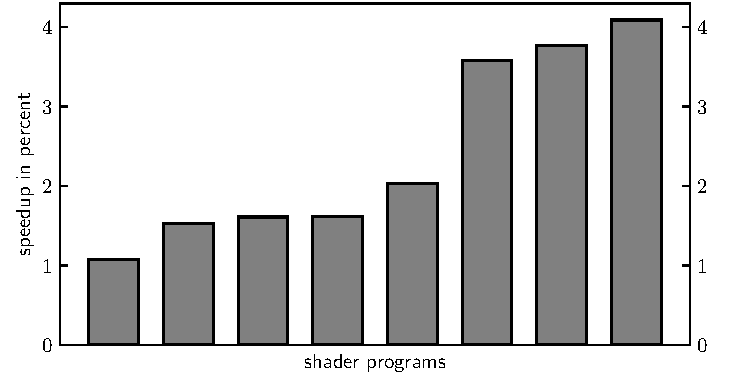
\includegraphics[width=\linewidth]{figures/qualcomm_plot.pdf}
\caption{Speedup on Qualcomm Adreno 530}
\label{fig:qualcommspeedup}
\end{figure}

\subsection{Polyhedral SCoPs}

    The polyhedral model allows compilers to utilize powerful mathematical
    reasoning to detect parallelism opportunities in sequential code and to
    implement sophisticated code transformations for well structured nested
    loops.
    It is currently applicable to Static Control Flow Parts (SCoPs) with affine
    data dependencies.
    Detecting SCoPs is fundamental for any later polyhedral optimization.

    Implementations of the polyhedral model may differ in their precise
    definition of SCoPs.
    We implemented SCoP detection functionality in CAnDL and compared against
    the Polly implementation in LLVM.
    We rely on the definition of Semantic SCoPs in \cite{Lengauer2012Polly}.
    The constraints for SCoPs can be broken into several components:

    \paragraph{Structured Control Flow}
    SCoPs require well structured control flow.
    Technically speaking, this means that every conditional jump within the
    corresponding piece of IR is accounted for by for loops and conditionals.
    We enforce this with the \texttt{collect} statement as demonstrated in
    \autoref{fig:collectexample}.
    We use \texttt{collect} with CAnDL programs \texttt{ForLoop} and
    \texttt{Conditional} that describe the control flow of for loops and
    conditionals and extract the involved conditional jump instructions.
    We then use another \texttt{collect} to verify that these are indeed all
    conditional jumps within the potential SCoP.

    Once we have established the control flow, we can use the iterators that are
    involved in the loops to define affine integer computations in the loop.
    This is done in a brute force fashion with a recursive constraint program.
    Using this analysis we then check that the iteration domain of all the for
    loops is well behaved, i.e.\ the boundaries are affine in the loop
    iterators.

    \paragraph{Affine Memory Access}
    We want to make sure that all memory access in the SCoP is affine.
    For this to be true we have to verify that for each load and store
    instruction, the base pointer is loop invariant and the index is calculated
    affinely.
    The loop invariant base pointer is easily guaranteed using the
    \texttt{LocalConst} program from \autoref{fig:localconstant}.

    Checking the index calculations is more involved and is again based on the
    \texttt{collect} method that was demonstrated in
    \autoref{fig:collectexample}.
    We use the \texttt{collect} construct to find all of the affine memory
    accesses in all the loop nests.
    We then use collect all \texttt{load} and \texttt{store} instructions and
    verify that both collections are identical.

    \paragraph{}
    We evaluated our detection of SCoPs on the PolyBench suite.
    For both our method as well as for Polly, we counted how many of the
    computational kernels in the benchmark suite are captured by the
    analysis.

\subsubsection{Results}

    As is visible in \autoref{fig:restable}, we capture all the SCoPs that Polly
    was able to detect.
    There is some postprocessing of the generated constraint solutions required
    to achieve this.
    Firstly, our results are not in the jscop format that Polly uses but contain
    the raw constraint solution as shown on the right side of \autoref{fig:gui}.
    Also, our CAnDL implementation does not merge consecutive outer level loops
    into SCoPs of maximum size.
    To compare the results, we extracted the detected loops from our report
    files, manually grouped them into maximum size SCoPs and verified that they
    fully cover the SCoPs detected by Polly.

    For lines of code, we compared our version with the amount of code in
    Polly's \texttt{ScopDetection.cpp} pass.
    We are able to detect the same number of SCoPs with much fewer lines of
    code.
    Note that the LoC count that we give for our SCoP program does not include
    all CAnDL code involved in the detection of polyhedral regions.
    We consider the code that is not specific to this idiom (such as loop
    structures) to be part of the CAnDL standard library.
    In the same way we did not account for e.g\ the ScalarEvolution pass when
    counting the lines for Polly.

    By having a high level representation of SCoPs, we allow polyhedral compiler
    researchers to explore the impact of relaxing or tightening the exact
    definition of SCoPs in a straightforward manner, enabling rapid prototyping.


\begin{figure}[h]
\centering
\begin{tabular}{|l||l|l|}
\hline
         & Polly & CAnDL \\
\hline
\hline
Lines of Code & 1903 & 45 \\ \hline
Detected in datamining & 2 & 2\\
Detected in Linear-algebra & 19 & 19\\
Detected in medley & 3 & 3\\
Detected in stencils & 6 & 6\\ \hline
%Compilation time & 24.4s+37.5s & 24.4s+12.7s \\ \hline
\hline
\end{tabular}
\caption{SCoPs detected Polly vs CAnDL}
\label{fig:restable}
\end{figure}



\chapter{Formalizing Idioms with CAnDL}
This chapter is based on ASAPLOS.


\chapter{Building a Fully integrated Idiom Specific Optimization Pipeline}
This chapter is based on LiLAC.
\section{Harnesses}
\section{Setup}
\section{Results}


\chapter{Conclusion}

\bibliography{../references}
\end{document}
